\documentclass[11pt,a4paper]{article}
\usepackage[margin=2cm]{geometry}
\usepackage[T1]{fontenc}\usepackage{tgheros}\renewcommand{\familydefault}{\sfdefault}
\usepackage{graphicx,booktabs,float,caption,amsmath,xcolor}
\usepackage[hidelinks]{hyperref}
\captionsetup{font=small,labelfont=bf}
\setlength{\parskip}{4pt}\setlength{\parindent}{0pt}
\setcounter{secnumdepth}{3}
\title{\textbf{PathSnap: GPS map-matching with a trained candidate classifier and an HMM decoder}\\[2pt]
\large UE24CS352A Machine Learning Hackathon --- Team 148 --- Technical report}
\author{Adyanth, Advitha, Sudhe, Tilak}
\date{19 November 2026}
\begin{document}
\maketitle

\begin{abstract}
We reconstruct the road route driven by a vehicle from its noisy GPS track. For every GPS point we generate the
nearby road arcs as candidates, score each (point, candidate) pair with a trained classifier, and decode one connected
route with a hidden Markov model solved by Viterbi. Ten classifiers from six families were compared with the same
trip-grouped cross-validation; a Bayesian-tuned LightGBM was selected by cross-validated Top-1. On the 10 held-out
STUDENT\_TEST trips the full pipeline matches \textbf{91.3\%} of GPS points to the correct arc
(classifier alone 88.0\%, rule baseline 83.2\%), raises route continuity from 0.867 to
0.930 and cuts route breaks from 653 to 259. On the 10 EVALUATOR
trips, scored by the API server, it reaches 91.3\%. A FastAPI server runs the pipeline and a Streamlit UI shows the
predicted route and the server-side scores.
\end{abstract}

\section{Problem and pipeline}
Each trip has a GPS track (longitude, latitude, time), its own road network (nodes and directed arcs) and, for
development trips, a reference route given as an ordered list of arc ids. The task is to output one arc per GPS
point. The pipeline is:
\begin{enumerate}\setlength\itemsep{0pt}
\item project the trip into its local UTM zone (all distances in metres);
\item generate candidate arcs within $R=60$\,m of each point, at most $K=30$ (fallback 150\,m);
\item compute 36 features per (point, candidate) pair from GPS and network geometry only;
\item score each pair with the exported classifier ($P(\text{candidate is the true arc})$);
\item decode a route with an HMM/Viterbi decoder over the candidate sets;
\item serve it through an API and a UI; evaluator scoring happens on the server after prediction.
\end{enumerate}
\textbf{Partitions.} TRAIN (80 trips) for fitting, cross-validation and all tuning; STUDENT\_TEST (10 trips) for
held-out comparison; EVALUATOR (10 trips) only on the API server. The loader refuses to read the evaluator partition
unless the API runs in serve mode, so it cannot leak into development. Seed 148 everywhere.

\section{Dataset understanding and exploratory data analysis}
\subsection{How we preprocessed the data}
\begin{enumerate}\setlength\itemsep{0pt}
\item \textbf{Quality checks} on both TRAIN and STUDENT\_TEST (Table~\ref{tab:quality}): missing files, NaN rows,
invalid or (0,0) coordinates, duplicate or backwards timestamps, time gaps, implied speeds, network integrity. No
rows are deleted; problems are flagged and handled downstream.
\item \textbf{Projection.} The trips lie in 25 different UTM zones. Each trip is projected to the UTM zone of its
median point; Euclidean distances on degrees are never used.
\item \textbf{Per-point labels.} The reference route is an arc sequence, not a label per point. We align points to
route arcs with a monotonic dynamic programme: the route position only moves forward, and the cost is
point-to-arc distance (capped at 100\,m) plus a heading-mismatch term. Median point-to-label distance is 4.75\,m.
Points more than 50\,m from their aligned arc (11.1\% of TRAIN, mostly three trips where the route covers only part of
the track; 0.14\% of STUDENT\_TEST) are flagged unreliable and excluded from training and scoring.
\item \textbf{Candidates.} A spatial index (STRtree) returns the arcs within $R$ of each point, at most $K$. $R=60$\,m
and $K=30$ were chosen on TRAIN from the miss rate (true arc not among the candidates) against candidate-set size
(Figure~\ref{fig:miss}): miss rate 0.029\% on TRAIN and 0\% on STUDENT\_TEST, about 12 candidates per point, 9\%
positives.
\end{enumerate}

\begin{table}[H]\centering\small
\caption{Missing-value and anomaly checks per partition (\texttt{scripts/inventory.py}, \texttt{scripts/eda.py}).}\label{tab:quality}
\resizebox{\ifdim\width>\linewidth\linewidth\else\width\fi}{!}{\begin{tabular}{lrr}\toprule
Check & TRAIN & STUDENT\_TEST \\ \midrule
Trips & 80 & 10 \\
GPS points & 208,417 & 19,160 \\
Missing files & 0 & 0 \\
NaN rows & 0 & 0 \\
Out-of-range coordinates & 0 & 0 \\
(0, 0) coordinates & 0 & 0 \\
Duplicate timestamps & 0 & 0 \\
Backwards timestamps & 0 & 0 \\
Time steps > 5 s & 1,216 & 44 \\
Longest time step (s) & 153,064 & 210 \\
Steps implying > 60 m/s & 546 & 2 \\
\bottomrule\end{tabular}}\end{table}

\subsection{What we observed}
\textbf{Missing values}: none --- every trip has all four files and there are no NaN, invalid or duplicate rows
(Table~\ref{tab:quality}, both partitions). \textbf{Sampling}: 96.5\% of TRAIN steps are exactly 1\,s, but 1,216 TRAIN steps
exceed 5\,s and the longest (42\,h, trip 00000090) is a parked vehicle, so the decoder must split on gaps.
\textbf{Speed outliers}: 546 TRAIN steps imply more than 60\,m/s, almost all in three trips and sustained (motorways),
not single spikes, so no point was removed. \textbf{Networks}: each trip has its own network (299--155,003 nodes,
649--307,392 arcs), so arc ids are local and the problem is framed per (point, candidate) pair rather than as a
global arc vocabulary. About 92\% of arcs have a reverse twin (two-way roads), so direction is a central difficulty.
\textbf{Routes}: in three TRAIN trips the reference route covers only part of the GPS path, which is why labels are
checked for reliability.

\begin{figure}[H]\centering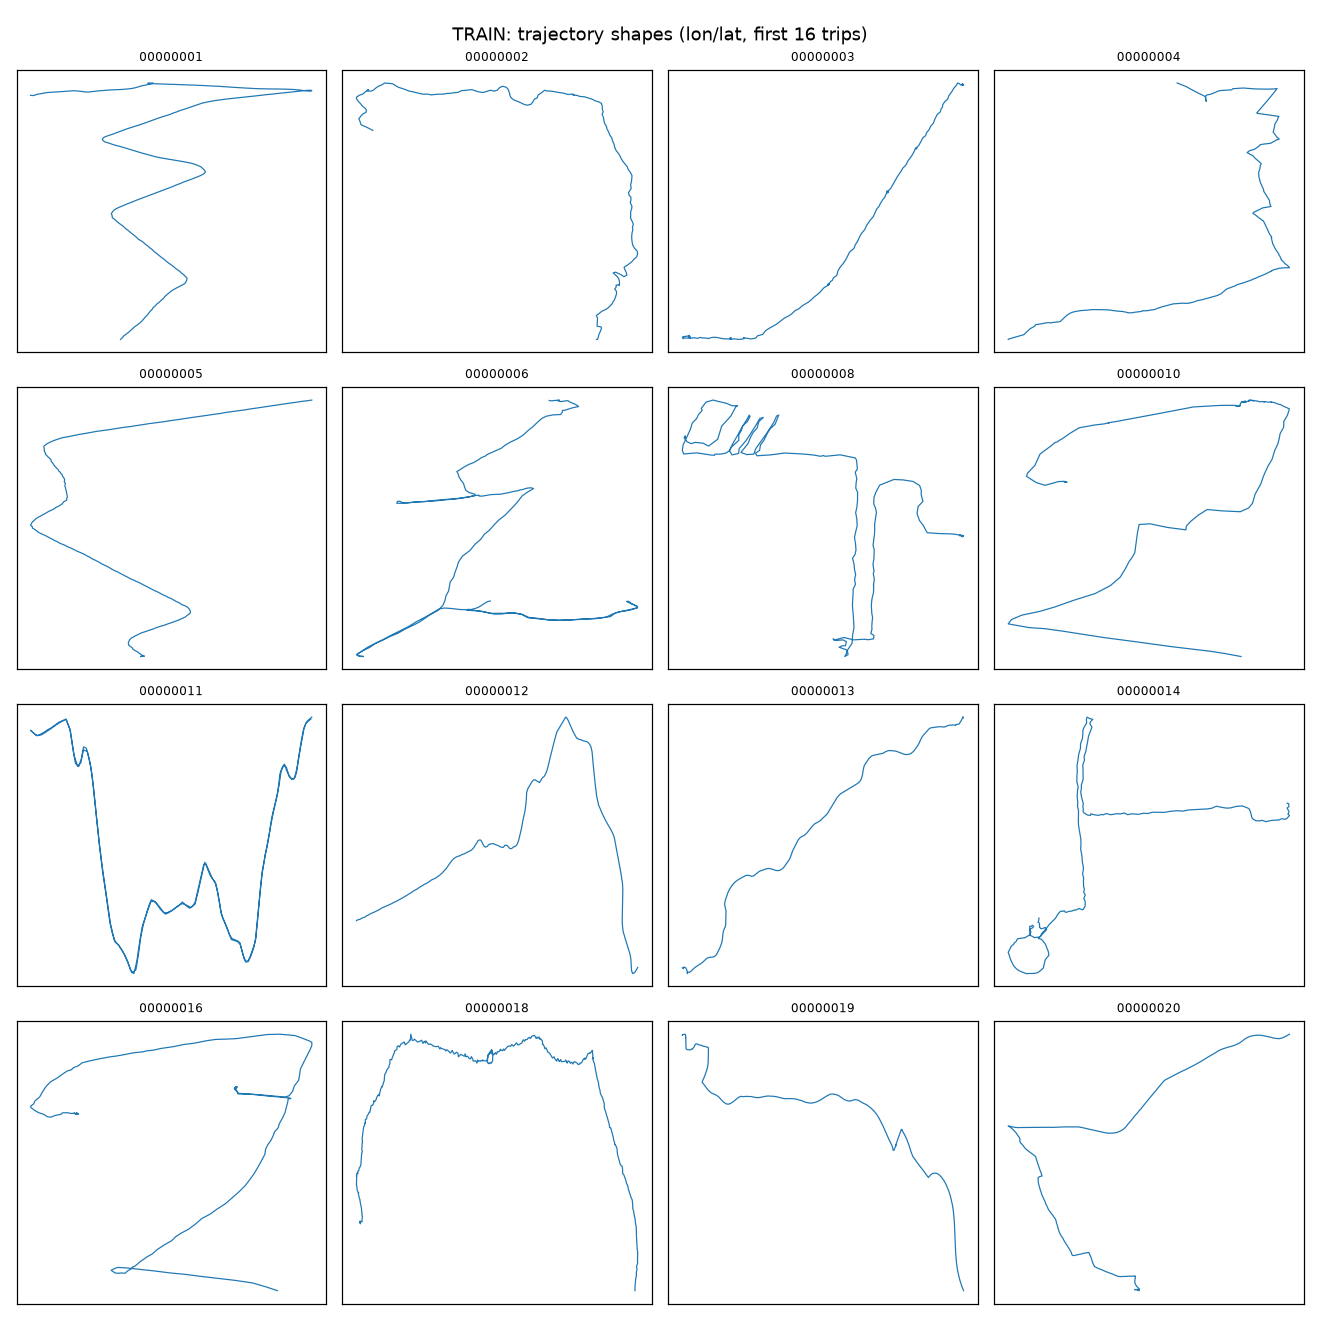
\includegraphics[width=0.78\linewidth]{../experiments/figures/eda_trajectories.png}
\caption{GPS trajectory shapes (TRAIN, first 16 trips).}\label{fig:traj}\end{figure}

\begin{figure}[H]\centering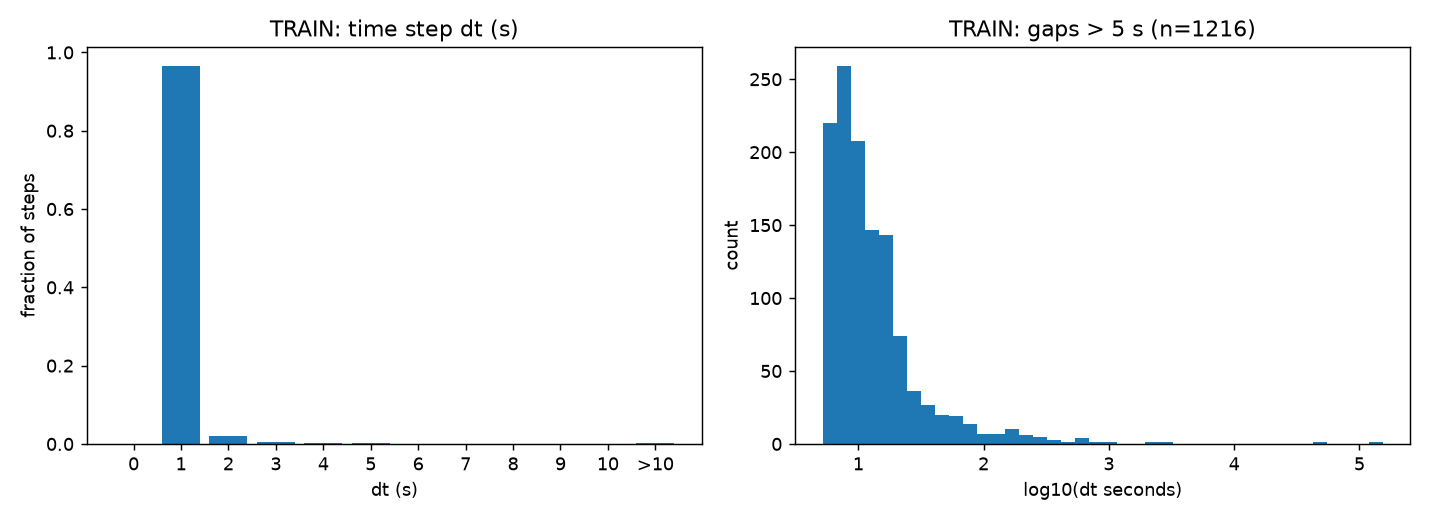
\includegraphics[width=0.8\linewidth]{../experiments/figures/eda_dt_hist.png}
\caption{Time steps between GPS points and the gaps above 5\,s (TRAIN).}\label{fig:dt}\end{figure}

\begin{figure}[H]\centering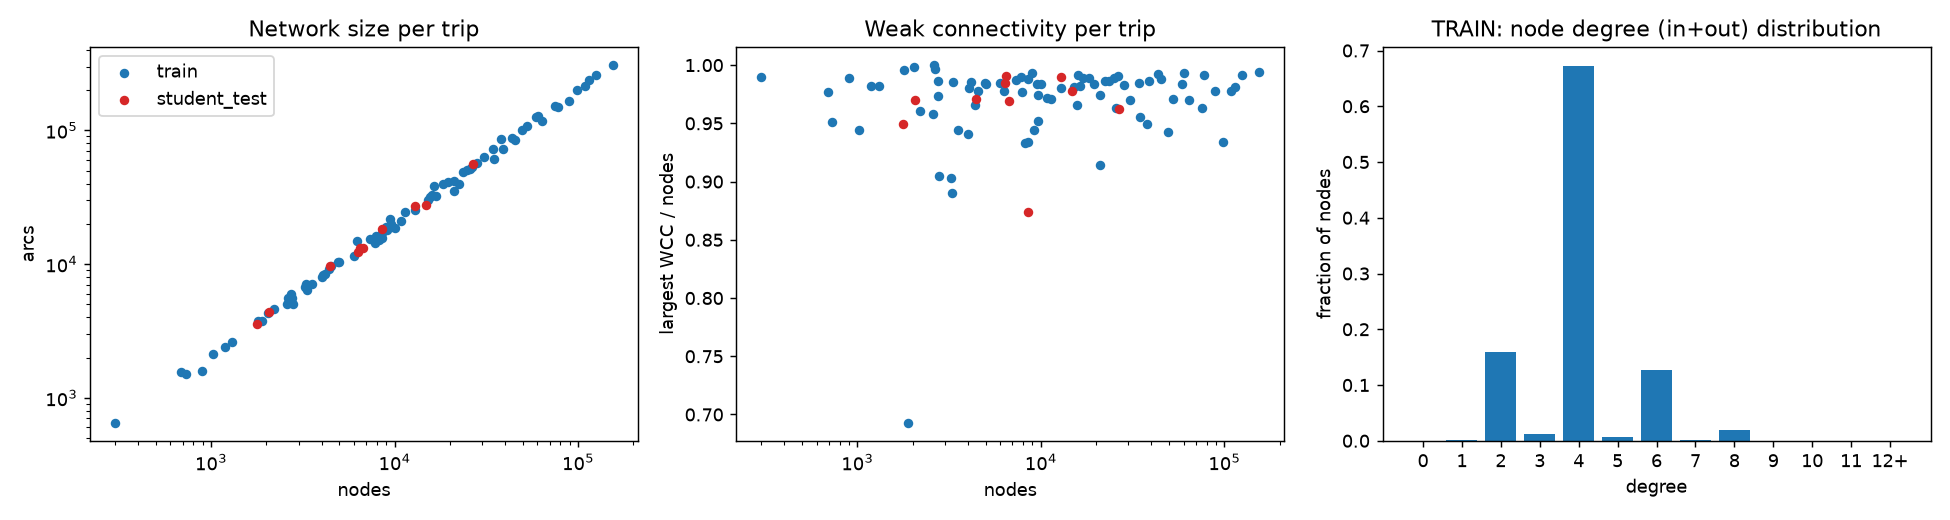
\includegraphics[width=\linewidth]{../experiments/figures/eda_network.png}
\caption{Road networks: size, weak connectivity and node degree per trip (TRAIN and STUDENT\_TEST).}\label{fig:net}\end{figure}

\begin{figure}[H]\centering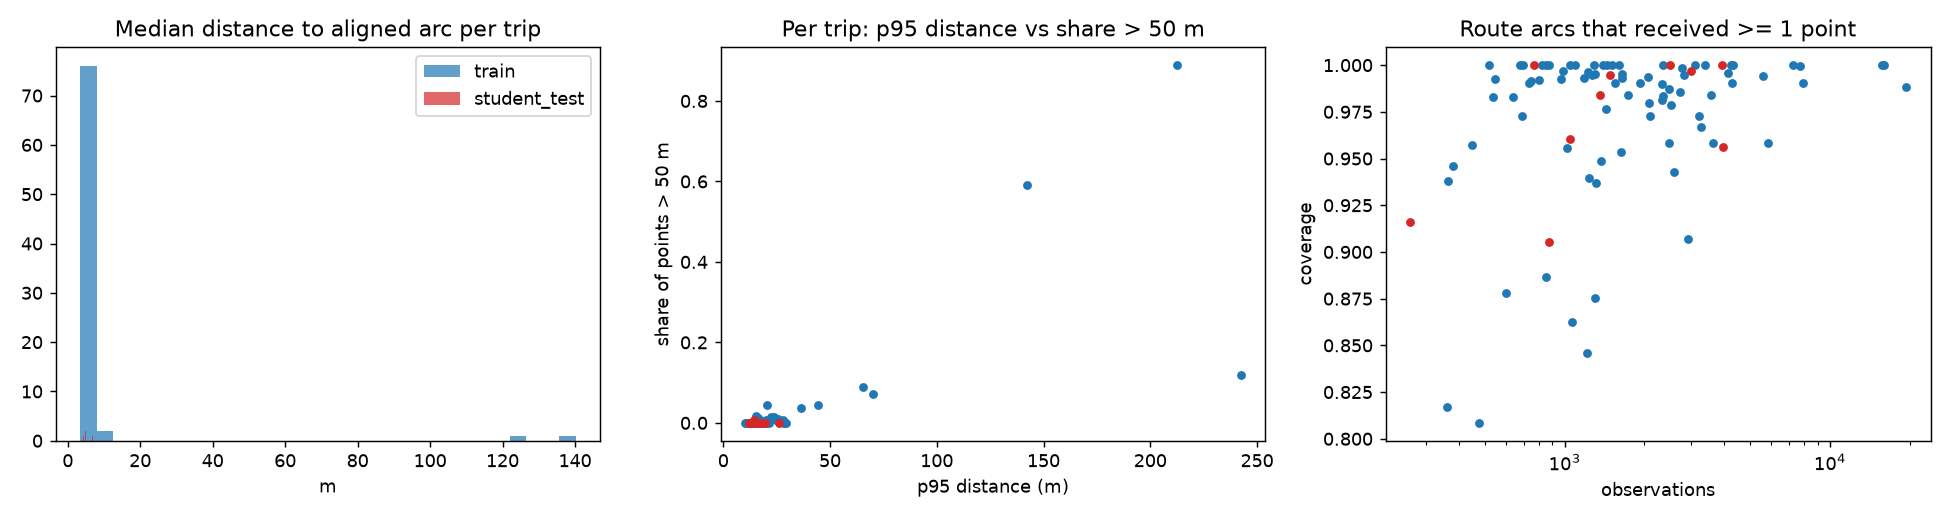
\includegraphics[width=\linewidth]{../experiments/figures/label_quality.png}
\caption{Quality of the derived labels per trip (TRAIN and STUDENT\_TEST).}\label{fig:labels}\end{figure}

\begin{figure}[H]\centering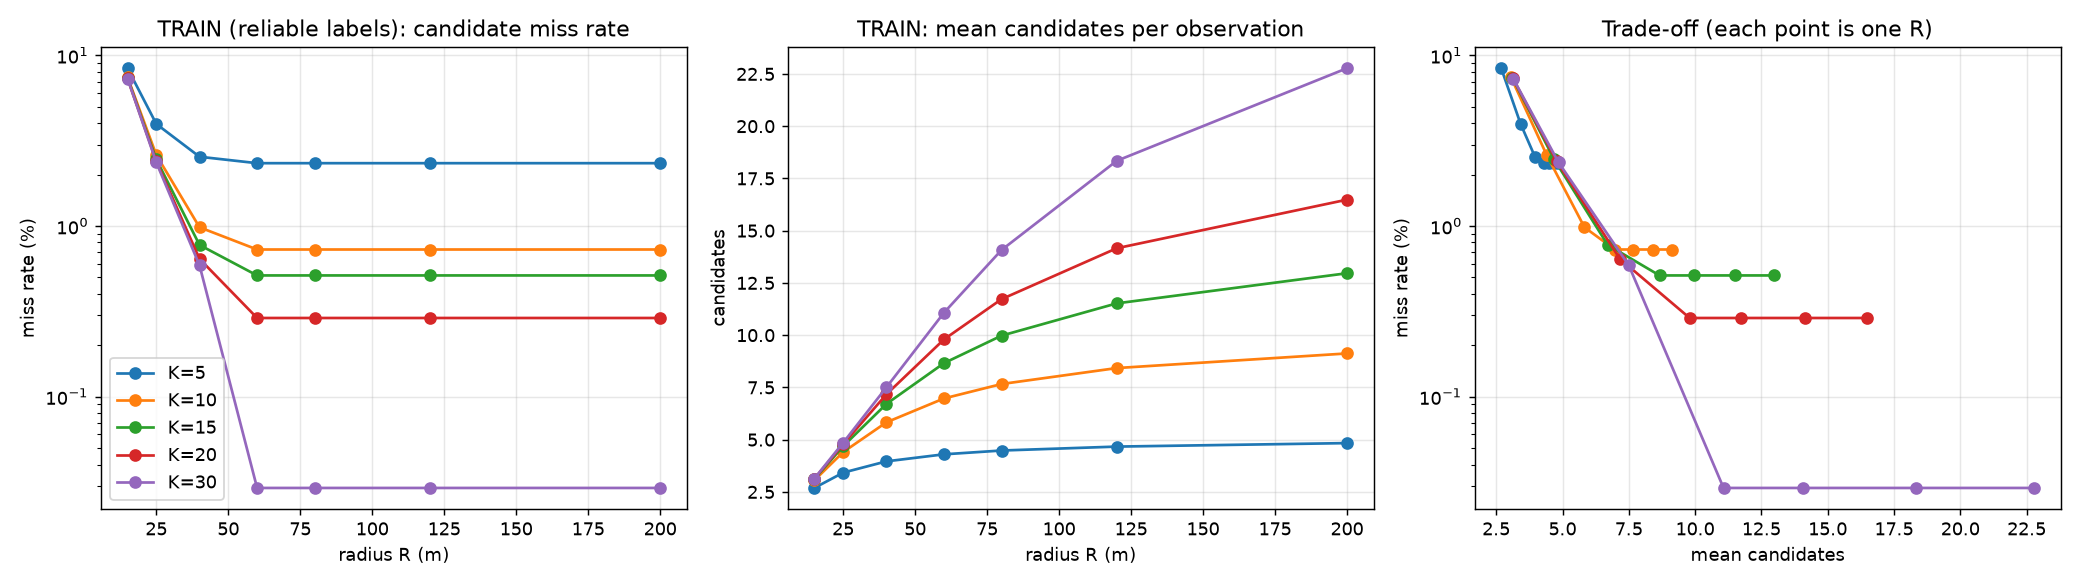
\includegraphics[width=\linewidth]{../experiments/figures/candidate_miss_rate.png}
\caption{Candidate miss rate and candidate count against radius $R$ (TRAIN).}\label{fig:miss}\end{figure}

\begin{figure}[H]\centering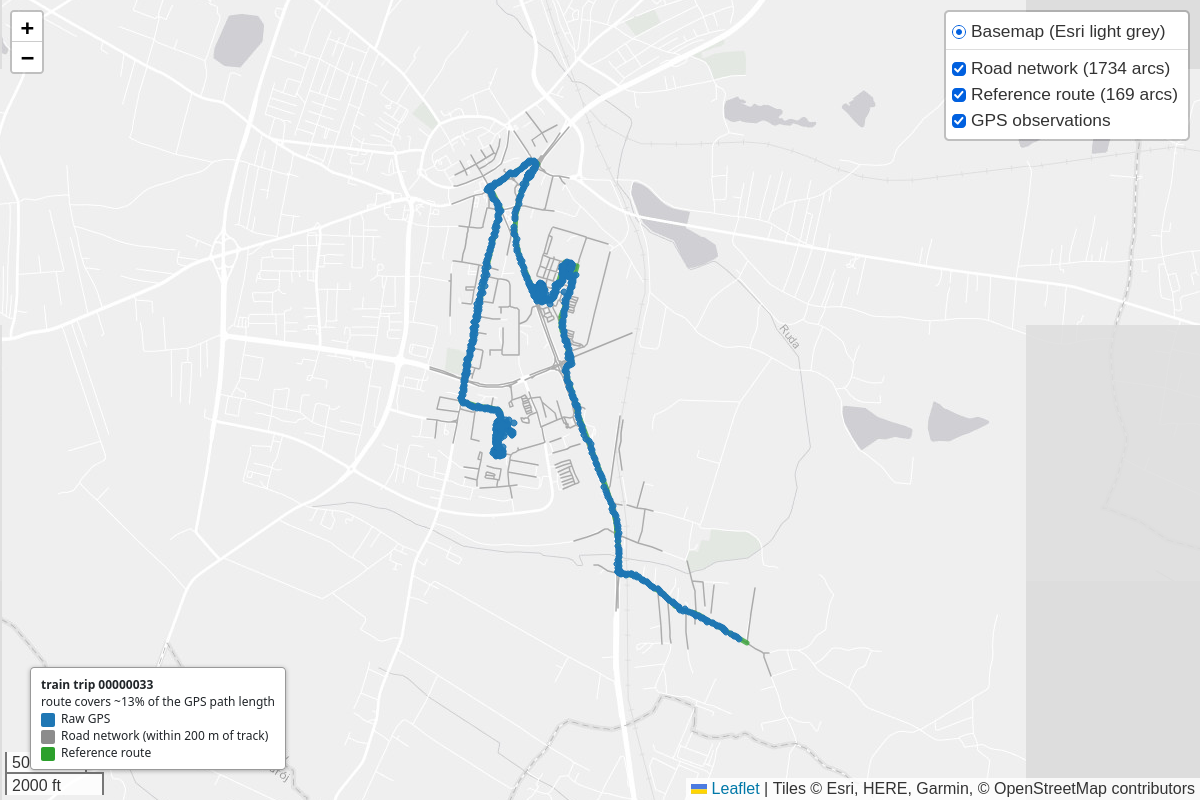
\includegraphics[width=0.75\linewidth]{figures/map_eda_train_00000033.png}
\caption{Folium EDA map, TRAIN trip 00000033: raw GPS (blue), road network within 200\,m (grey), reference route (green). The route covers only part of the track.}\label{fig:eda_map}\end{figure}


\subsection{Features and why we chose them}
All 36 features use only GPS and network geometry (never labels), grouped by what they capture:
\emph{distance} (point-to-arc distance, rank among the candidates, gap to the closest, projection position) because the
true arc is usually the closest; \emph{direction} (cosine between GPS heading and arc bearing, also for the previous and
next points) because half the candidate rows are reverse twins with identical distance; \emph{context} (distance of
the neighbouring points to the same arc) because one noisy point can sit near the wrong road while its neighbours do
not; \emph{motion} (time steps, speeds, acceleration, turn angle); \emph{network} (arc length, node degrees,
reverse-twin flag); \emph{sequence} (agreement with the neighbours' best arc) and \emph{density} (number of nearby
candidates). An ablation with Logistic Regression shows what each group adds on STUDENT\_TEST: distance and density only
0.546, plus direction 0.843, all 36 features
0.858 Top-1.

\section{Model experimentation and comparison}
\subsection{Overall comparison and final model}
Every model goes through one shared harness (\texttt{src/pathsnap/harness.py}): the same 36 features, the same trip
folds (GroupKFold(5) by trip, saved in \texttt{experiments/results/cv\_folds.csv}, so no trip is in both training and
validation), the same metrics and the same STUDENT\_TEST scoring. The \textbf{primary metric is observation-level Top-1}:
is the highest-scored candidate of a point its label arc? It needs no threshold and is exactly what the route needs.
Candidate-level macro F1 (threshold 0.5) and log loss are reported with it.

\begin{table}[H]\centering\scriptsize
\caption{Model comparison, sorted by the selection metric (CV Top-1, Table~\ref{tab:cv}). CV = 5-fold GroupKFold by trip on TRAIN; Top-1, continuity, macro F1 and log loss on STUDENT\_TEST. Top-1 is observation-level accuracy. Continuity is for the classifier-only route (the HMM is in Section~5). Inference = scoring time per trip.}\label{tab:comp}
\begin{tabular}{p{2.3cm}p{2.2cm}p{3.6cm}ccccccc}\toprule
Model & Family & Key configuration & CV macro F1 & Top-1 & Route cont. & Macro F1 & Log loss & ms/trip \\ \midrule
LightGBM, Bayesian-tuned & gradient boosting (LightGBM, Bayesian-tuned) & n\_estimators=800, learning\_rate=0.01413, num\_leaves=254, min\_child\_samples=20 & 0.925 $\pm$ 0.019 & 0.8796 & 0.867 & 0.933 & 0.047 & 169.2 \\
LightGBM (untuned) & gradient boosting (LightGBM) & n\_estimators=400, learning\_rate=0.05, num\_leaves=63, min\_child\_samples=50 & 0.925 $\pm$ 0.018 & 0.8787 & 0.867 & 0.933 & 0.047 & 37.0 \\
XGBoost & gradient boosting (XGBoost) & n\_estimators=400, learning\_rate=0.05, max\_depth=8 & 0.924 $\pm$ 0.019 & 0.8809 & 0.869 & 0.934 & 0.047 & 10.5 \\
HistGradientBoosting (scikit-learn) & gradient boosting (sklearn HistGB) & max\_iter=300, learning\_rate=0.1, max\_leaf\_nodes=63 & 0.923 $\pm$ 0.018 & 0.8773 & 0.863 & 0.931 & 0.048 & 24.0 \\
Random Forest & bagged trees (Random Forest) & n\_estimators=120, max\_depth=18, min\_samples\_leaf=2 & 0.910 $\pm$ 0.019 & 0.8735 & 0.865 & 0.914 & 0.070 & 39.1 \\
Extra Trees & bagged trees (Extra Trees) & n\_estimators=120, max\_depth=18, min\_samples\_leaf=2 & 0.900 $\pm$ 0.019 & 0.8669 & 0.844 & 0.905 & 0.086 & 40.7 \\
Decision Tree & single tree & max\_depth=8, min\_samples\_leaf=10 & 0.871 $\pm$ 0.019 & 0.8653 & 0.831 & 0.875 & 0.109 & 0.6 \\
Logistic Regression & linear / probabilistic & C=1, penalty=l2, class\_weight=balanced & 0.861 $\pm$ 0.013 & 0.8580 & 0.804 & 0.861 & 0.128 & 0.7 \\
SGD classifier (logistic loss) & linear (SGD, log loss) & alpha=0.0001, penalty=l2, class\_weight=balanced & 0.862 $\pm$ 0.013 & 0.8555 & 0.798 & 0.861 & 0.128 & 0.8 \\
Gaussian Naive Bayes & probabilistic (generative) & var\_smoothing=1e-09 & 0.812 $\pm$ 0.013 & 0.7720 & 0.779 & 0.806 & 0.836 & 1.6 \\
\bottomrule\end{tabular}\end{table}

\begin{table}[H]\centering\small
\caption{Cross-validation detail (TRAIN). Train$-$CV F1 is the over/underfitting evidence used in Section~3.2.}\label{tab:cv}
\resizebox{\ifdim\width>\linewidth\linewidth\else\width\fi}{!}{\begin{tabular}{lcccccc}\toprule
Model & CV Top-1 & std & CV log loss & Train-fold F1 & Train$-$CV F1 & Fit (s) \\ \midrule
LightGBM, Bayesian-tuned & 0.8651 & 0.0355 & 0.0638 & 0.963 & +0.038 & 41 \\
LightGBM (untuned) & 0.8639 & 0.0350 & 0.0637 & 0.952 & +0.028 & 12 \\
XGBoost & 0.8632 & 0.0358 & 0.0642 & 0.956 & +0.031 & 14 \\
HistGradientBoosting (scikit-learn) & 0.8627 & 0.0348 & 0.0649 & 0.957 & +0.034 & 16 \\
Random Forest & 0.8624 & 0.0371 & 0.0852 & 0.940 & +0.031 & 101 \\
Extra Trees & 0.8600 & 0.0369 & 0.0989 & 0.917 & +0.017 & 50 \\
Decision Tree & 0.8557 & 0.0356 & 0.1306 & 0.877 & +0.006 & 32 \\
Logistic Regression & 0.8534 & 0.0354 & 0.1412 & 0.861 & +0.000 & 10 \\
SGD classifier (logistic loss) & 0.8532 & 0.0354 & 0.1392 & 0.862 & +0.000 & 6 \\
Gaussian Naive Bayes & 0.7881 & 0.0412 & 0.8994 & 0.812 & -0.000 & 1 \\
\bottomrule\end{tabular}}\end{table}

Rule baselines (no learning, STUDENT\_TEST): rule\_nearest\_arc (heading\_weight\_m=0): Top-1 0.530; rule\_nearest\_heading (heading\_weight\_m=20 (chosen on train)): Top-1 0.832.

\textbf{Final model: Bayesian-tuned LightGBM} (\texttt{advitha\_lgbm\_tuned}), chosen by the rule fixed before tuning: highest
CV Top-1. It also has the best CV macro F1 and the lowest STUDENT\_TEST log loss, i.e. the best-calibrated
probabilities, which matters because the HMM uses them as emissions. XGBoost is marginally higher on STUDENT\_TEST
Top-1, but the gap (about 25 of 19,133 points) is far inside the fold-to-fold spread, and choosing on a 10-trip test set
would be selecting on the test data. The boosting models are statistically tied; the features matter more than the
library. The cost is speed: about 169\,ms per trip for scoring, still far below a second.

\subsection{Per model}
\subsubsection{LightGBM, Bayesian-tuned (final model)}
\textit{Trained by Advitha, Adyanth; script \texttt{scripts/models/advitha\_lgbm\_tuned.py}.}

\textbf{A1. Why suitable.} Same algorithm as the untuned LightGBM below; the hyperparameters come from the 40-trial Optuna search of Section~4. It is the model with the highest cross-validated Top-1, so it is the one exported to the API and used as the HMM emission model.

\textbf{A2. Strengths and limitations.} Strengths: best CV Top-1 and CV macro F1 of all ten models and the lowest STUDENT\_TEST log loss, i.e. the best-calibrated probabilities, which the HMM uses directly. Limitations: 254 leaves and 800 trees make it the slowest model to score (169\,ms per trip, 4.6$\times$ the untuned one) and it has the largest train/CV gap.

\textbf{B5. Hyperparameters (initial values).} \texttt{objective} = binary, \texttt{n\_estimators} = 800, \texttt{learning\_rate} = 0.01413, \texttt{num\_leaves} = 254, \texttt{min\_child\_samples} = 20, \texttt{subsample} = 0.9151, \texttt{colsample\_bytree} = 0.7893, \texttt{reg\_lambda} = 0.04488, \texttt{reg\_alpha} = 1.524 (from Optuna, optuna study lgbm\_top1\_v1, trial 32).

\textbf{B6. Loss / objective.} Binary log loss (cross-entropy) on (point, candidate) rows, minimised by gradient boosting with L1 (1.52) and L2 (0.045) penalties on the leaf weights.

\textbf{C7--C8. STUDENT\_TEST results.} Top-1 0.8796, macro F1 0.9334, log loss 0.0470, classifier-only route continuity 0.867 (CV Top-1 0.8651 $\pm$ 0.0355).

\textbf{C9. Over- or underfitting.} Mild overfitting. Train-fold macro F1 is 0.963 against 0.925 in CV (gap +0.038, the largest of all models). The loss curve on a held-out fold (Figure~\ref{fig:loss}) shows the validation loss flat from about iteration 549 while the training loss keeps falling (0.0335 vs 0.0467 at the end). The validation loss does not rise, so the extra trees cost time but not accuracy.
\subsubsection{LightGBM (untuned)}
\textit{Trained by Advitha; script \texttt{scripts/models/advitha\_lgbm.py}.}

\textbf{A1. Why suitable.} Each GPS point has 1--30 candidate arcs and the question is which one is right; this is a tabular binary problem with strong feature interactions (a near arc is only right if its direction also matches and the neighbouring points agree). Gradient-boosted trees learn such interactions without scaling, handle the 1:10 class ratio well and give usable probabilities. It was the first model trained on the shared feature table and served as the reference for tuning.

\textbf{A2. Strengths and limitations.} Strengths: second-best CV Top-1, fast to fit (12\,s on 2 million rows) and to score (37\,ms per trip). Limitations: many hyperparameters; leaf-wise growth can overfit small groups of rows, which is why min\_child\_samples and subsampling are set.

\textbf{B5. Hyperparameters (initial values).} \texttt{objective} = binary, \texttt{n\_estimators} = 400, \texttt{learning\_rate} = 0.05, \texttt{num\_leaves} = 63, \texttt{min\_child\_samples} = 50, \texttt{subsample} = 0.8, \texttt{colsample\_bytree} = 0.8, \texttt{reg\_lambda} = 1.

\textbf{B6. Loss / objective.} Binary log loss, gradient boosting with L2 penalty 1 on leaf weights.

\textbf{C7--C8. STUDENT\_TEST results.} Top-1 0.8787, macro F1 0.9330, log loss 0.0473, classifier-only route continuity 0.867 (CV Top-1 0.8639 $\pm$ 0.0350).

\textbf{C9. Over- or underfitting.} Slight overfitting: train-fold macro F1 0.952 vs CV 0.925 (gap +0.028). On the held-out fold the validation loss is lowest at iteration 352 of 400 and stays flat after it (Figure~\ref{fig:loss}). CV Top-1 varies by $\pm$0.035 across folds, so the trips, not the model, dominate the variance.
\subsubsection{XGBoost}
\textit{Trained by Advitha; script \texttt{scripts/models/advitha\_xgb.py}.}

\textbf{A1. Why suitable.} A second boosting implementation, grown depth-wise with second-order (Newton) updates, to check whether the result depends on the LightGBM library or on the features.

\textbf{A2. Strengths and limitations.} Strengths: the highest STUDENT\_TEST Top-1 (0.8809) and fast inference (11\,ms per trip). Limitations: slightly lower CV Top-1 than both LightGBMs; depth-wise trees of depth 8 need more trees to model the same interactions.

\textbf{B5. Hyperparameters (initial values).} \texttt{objective} = binary:logistic, \texttt{n\_estimators} = 400, \texttt{learning\_rate} = 0.05, \texttt{max\_depth} = 8, \texttt{min\_child\_weight} = 5, \texttt{subsample} = 0.8, \texttt{colsample\_bytree} = 0.8, \texttt{reg\_lambda} = 1, \texttt{tree\_method} = hist.

\textbf{B6. Loss / objective.} Regularised binary log loss (objective binary:logistic) with L2 penalty 1, histogram tree method.

\textbf{C7--C8. STUDENT\_TEST results.} Top-1 0.8809, macro F1 0.9337, log loss 0.0472, classifier-only route continuity 0.869 (CV Top-1 0.8632 $\pm$ 0.0358).

\textbf{C9. Over- or underfitting.} Slight overfitting: train-fold F1 0.956 vs CV 0.924 (gap +0.031). Validation loss is lowest at iteration 223 of 400 and flat afterwards (Figure~\ref{fig:loss}). Its STUDENT\_TEST lead over the tuned LightGBM is about 25 of 19,133 points, far inside the fold-to-fold spread, so we did not select on it.
\subsubsection{HistGradientBoosting (scikit-learn)}
\textit{Trained by Advitha; script \texttt{scripts/models/advitha\_hgb.py}.}

\textbf{A1. Why suitable.} The scikit-learn histogram boosting implementation, a third boosting variant with no extra dependency, to confirm that the three boosting libraries agree.

\textbf{A2. Strengths and limitations.} Strengths: ties with the other boosting models (CV Top-1 0.8627) and is simple to deploy. Limitations: slightly lower STUDENT\_TEST Top-1 and higher log loss than LightGBM and XGBoost; the larger learning rate (0.1) gives a coarser fit.

\textbf{B5. Hyperparameters (initial values).} \texttt{loss} = log\_loss, \texttt{max\_iter} = 300, \texttt{learning\_rate} = 0.1, \texttt{max\_leaf\_nodes} = 63, \texttt{min\_samples\_leaf} = 50, \texttt{l2\_regularization} = 1, \texttt{early\_stopping} = False.

\textbf{B6. Loss / objective.} Binary log loss, gradient boosting with L2 regularisation 1; early stopping off so every model sees the same data.

\textbf{C7--C8. STUDENT\_TEST results.} Top-1 0.8773, macro F1 0.9312, log loss 0.0481, classifier-only route continuity 0.863 (CV Top-1 0.8627 $\pm$ 0.0348).

\textbf{C9. Over- or underfitting.} Slight overfitting: train-fold F1 0.957 vs CV 0.923 (gap +0.034), the same pattern as the other boosting models. With early stopping off no per-iteration history was recorded for this model.
\subsubsection{Random Forest}
\textit{Trained by Sudhe; script \texttt{scripts/models/sudhe\_random\_forest.py}.}

\textbf{A1. Why suitable.} Bagging is a different way to build a strong tree ensemble: deep trees on bootstrap samples with random feature subsets, averaged. It tests whether variance reduction alone reaches the boosting result.

\textbf{A2. Strengths and limitations.} Strengths: robust, few hyperparameters, CV Top-1 0.8624, close to boosting. Limitations: probabilities are less calibrated (log loss 0.070 vs 0.047 for boosting), it is the slowest model to fit (101\,s) and the balanced class weights shift the probabilities.

\textbf{B5. Hyperparameters (initial values).} \texttt{n\_estimators} = 120, \texttt{max\_depth} = 18, \texttt{min\_samples\_leaf} = 2, \texttt{class\_weight} = balanced.

\textbf{B6. Loss / objective.} No global loss: each tree greedily maximises the Gini impurity decrease at each split; balanced class weights.

\textbf{C7--C8. STUDENT\_TEST results.} Top-1 0.8735, macro F1 0.9139, log loss 0.0704, classifier-only route continuity 0.865 (CV Top-1 0.8624 $\pm$ 0.0371).

\textbf{C9. Over- or underfitting.} Moderate variance: train-fold F1 0.940 vs CV 0.910 (gap +0.031). Depth 18 with leaves of 2 rows lets single trees memorise, and averaging 120 of them only partly removes it.
\subsubsection{Extra Trees}
\textit{Trained by Sudhe; script \texttt{scripts/models/sudhe\_extra\_trees.py}.}

\textbf{A1. Why suitable.} Like Random Forest, but split thresholds are drawn at random, which reduces variance further and fits faster; a check of how much the exact split points matter.

\textbf{A2. Strengths and limitations.} Strengths: smaller train/CV gap than Random Forest, faster to fit (50\,s). Limitations: random thresholds blur the sharp distance and heading cut-offs that matter here, so Top-1 and log loss (0.086) are worse than Random Forest.

\textbf{B5. Hyperparameters (initial values).} \texttt{n\_estimators} = 120, \texttt{max\_depth} = 18, \texttt{min\_samples\_leaf} = 2, \texttt{class\_weight} = balanced.

\textbf{B6. Loss / objective.} Gini impurity per split with random thresholds; balanced class weights.

\textbf{C7--C8. STUDENT\_TEST results.} Top-1 0.8669, macro F1 0.9048, log loss 0.0862, classifier-only route continuity 0.844 (CV Top-1 0.8600 $\pm$ 0.0369).

\textbf{C9. Over- or underfitting.} Low variance, slight underfitting relative to Random Forest: gap +0.017 (train 0.917, CV 0.900), but CV macro F1 is 0.009 below Random Forest.
\subsubsection{Decision Tree}
\textit{Trained by Sudhe; script \texttt{scripts/models/sudhe\_decision\_tree.py}.}

\textbf{A1. Why suitable.} The single interpretable tree is the baseline that shows what the ensembles add; its first splits (distance rank, heading cosine) confirm which features carry the signal.

\textbf{A2. Strengths and limitations.} Strengths: fastest inference (0.6\,ms per trip) and readable rules; already 0.865 Top-1. Limitations: piecewise-constant probabilities (log loss 0.109) are poor HMM emissions and the depth limit caps accuracy.

\textbf{B5. Hyperparameters (initial values).} \texttt{max\_depth} = 8, \texttt{min\_samples\_split} = 20, \texttt{min\_samples\_leaf} = 10, \texttt{class\_weight} = balanced.

\textbf{B6. Loss / objective.} Gini impurity decrease per split; balanced class weights.

\textbf{C7--C8. STUDENT\_TEST results.} Top-1 0.8653, macro F1 0.8746, log loss 0.1090, classifier-only route continuity 0.831 (CV Top-1 0.8557 $\pm$ 0.0356).

\textbf{C9. Over- or underfitting.} Underfitting, not overfitting: depth 8 and leaves of at least 10 rows give a small gap (+0.006; train 0.877, CV 0.871) but CV macro F1 is 0.05 below boosting.
\subsubsection{Logistic Regression}
\textit{Trained by Adyanth; script \texttt{scripts/models/adyanth\_logreg.py}.}

\textbf{A1. Why suitable.} The simplest probabilistic classifier: a linear score of the 36 features. It shows how far the hand-made features go without learned interactions, and its coefficients are easy to explain. We also used it for the feature ablation in Section~2.

\textbf{A2. Strengths and limitations.} Strengths: trains in 10\,s, scores in under 1\,ms per trip, stable across folds (CV F1 std 0.013, the lowest). Limitations: a linear boundary cannot express rules such as ``close \emph{and} same direction''; balanced weights make the probabilities less calibrated (log loss 0.128).

\textbf{B5. Hyperparameters (initial values).} \texttt{C} = 1, \texttt{penalty} = l2, \texttt{class\_weight} = balanced, \texttt{solver} = lbfgs, \texttt{max\_iter} = 2000, \texttt{scaler} = standard.

\textbf{B6. Loss / objective.} Class-weighted binary cross-entropy with an L2 penalty (C = 1), solved by L-BFGS; features standardised inside the pipeline so each fold refits the scaler.

\textbf{C7--C8. STUDENT\_TEST results.} Top-1 0.8580, macro F1 0.8606, log loss 0.1282, classifier-only route continuity 0.804 (CV Top-1 0.8534 $\pm$ 0.0354).

\textbf{C9. Over- or underfitting.} Underfitting (high bias): train-fold and CV macro F1 are equal (0.861 vs 0.861, gap +0.000) and both are about 0.06 below boosting. More data would not help; more model capacity does.
\subsubsection{SGD classifier (logistic loss)}
\textit{Trained by Adyanth; script \texttt{scripts/models/adyanth\_sgd.py}.}

\textbf{A1. Why suitable.} The same linear model as Logistic Regression fitted by stochastic gradient descent, to see whether an iterative solver that scales to more data changes the result.

\textbf{A2. Strengths and limitations.} Strengths: fastest to fit of the linear models (6\,s), same accuracy as Logistic Regression. Limitations: sensitive to feature scale and the learning-rate schedule; same linear limits.

\textbf{B5. Hyperparameters (initial values).} \texttt{loss} = log\_loss, \texttt{penalty} = l2, \texttt{alpha} = 0.0001, \texttt{class\_weight} = balanced, \texttt{max\_iter} = 100, \texttt{tol} = 0.0001, \texttt{learning\_rate} = optimal, \texttt{scaler} = standard.

\textbf{B6. Loss / objective.} Class-weighted logistic loss with L2 penalty $\alpha$ = 0.0001, minimised by SGD with the ``optimal'' learning-rate schedule; standardised features.

\textbf{C7--C8. STUDENT\_TEST results.} Top-1 0.8555, macro F1 0.8612, log loss 0.1281, classifier-only route continuity 0.798 (CV Top-1 0.8532 $\pm$ 0.0354).

\textbf{C9. Over- or underfitting.} Underfitting, like Logistic Regression: gap +0.000 (train 0.862, CV 0.862). In the per-epoch curves (Figure~\ref{fig:loss}) the validation loss is lowest after epoch 2 (0.1019) and then fluctuates up to 0.1122 by epoch 30, while the training loss stays higher (0.1415). Training loss never falls below validation loss, so this is noise from the stochastic updates, not memorisation; a linear model has no capacity to overfit 2 million rows.
\subsubsection{Gaussian Naive Bayes}
\textit{Trained by Adyanth; script \texttt{scripts/models/adyanth\_gnb.py}.}

\textbf{A1. Why suitable.} A generative baseline: it models each feature per class as a Gaussian and assumes independence, which is quick to fit and shows the cost of ignoring feature correlations.

\textbf{A2. Strengths and limitations.} Strengths: fits in about a second, no tuning. Limitations: several features are strongly correlated (distance, distance rank, distance to the nearest candidate; heading cosines of neighbouring points), so the independence assumption multiplies the same evidence and the model is over-confident: log loss 0.836, 18$\times$ boosting, Top-1 0.772.

\textbf{B5. Hyperparameters (initial values).} \texttt{var\_smoothing} = 1e-09, \texttt{priors} = empirical, \texttt{scaler} = standard.

\textbf{B6. Loss / objective.} No iterative loss: class priors and per-class feature means and variances by maximum likelihood (var\_smoothing 1e-09).

\textbf{C7--C8. STUDENT\_TEST results.} Top-1 0.7720, macro F1 0.8061, log loss 0.8360, classifier-only route continuity 0.779 (CV Top-1 0.7881 $\pm$ 0.0412).

\textbf{C9. Over- or underfitting.} Underfitting: train-fold F1 0.812 equals CV 0.812 (gap -0.000); the error comes from the wrong independence assumption, not from too little data.


\subsection{Model visualisations}
\begin{figure}[H]\centering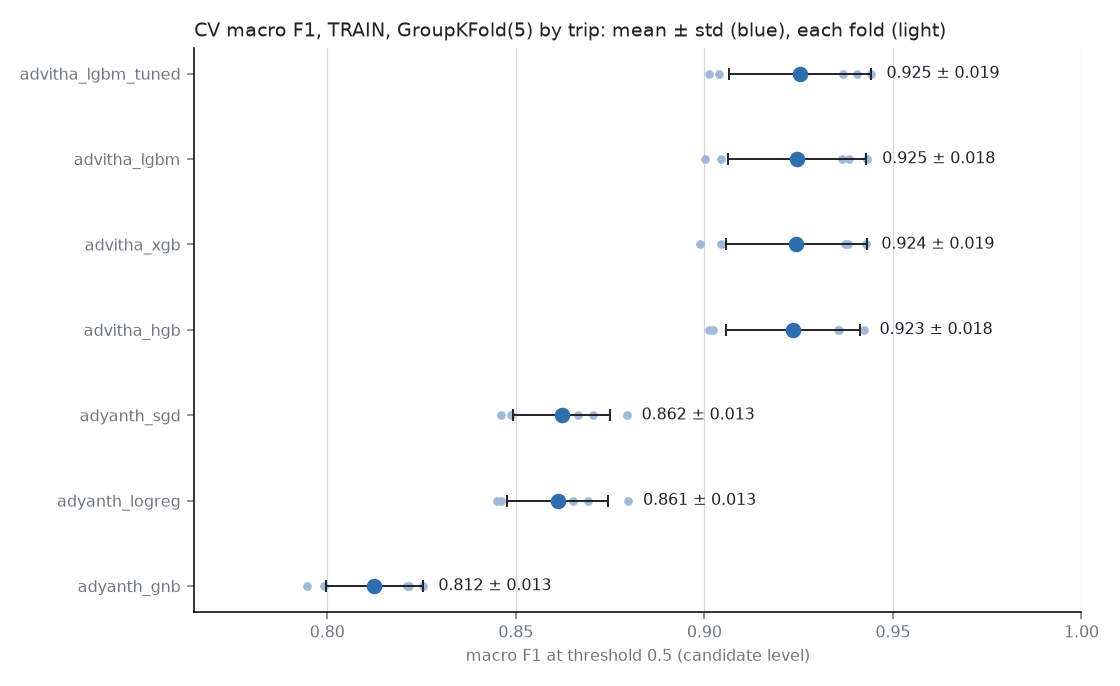
\includegraphics[width=0.85\linewidth]{../experiments/figures/cv_macro_f1.png}
\caption{CV macro F1 per model (TRAIN): mean $\pm$ std over the 5 folds, each fold shown.}\label{fig:cvf1}\end{figure}

\begin{figure}[H]\centering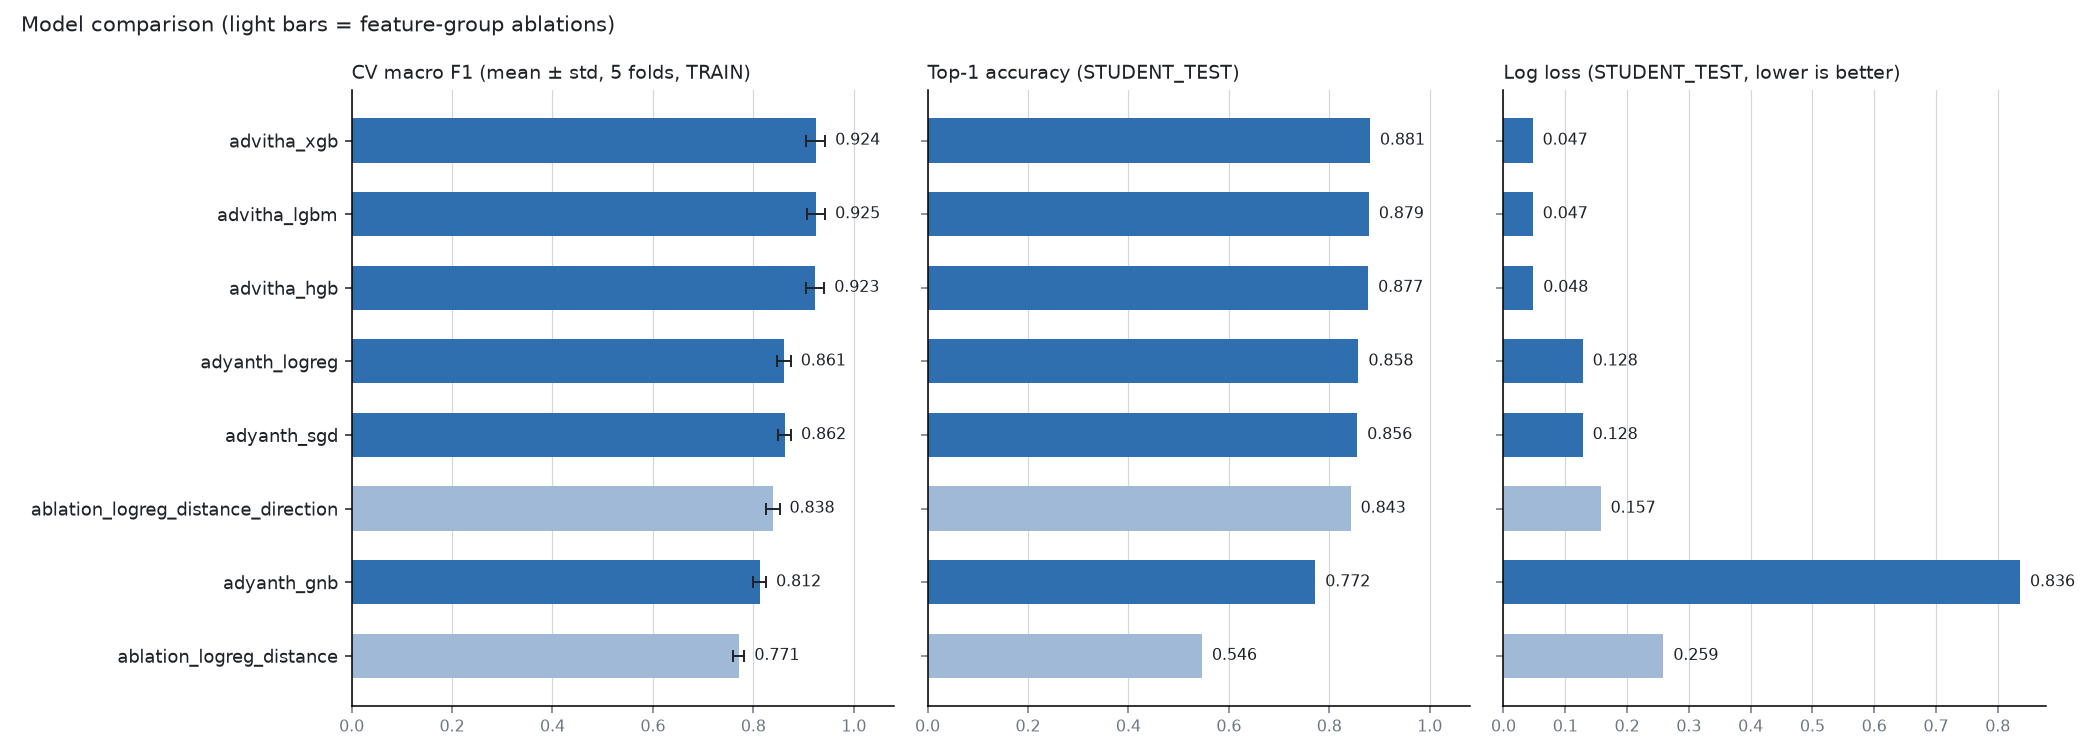
\includegraphics[width=\linewidth]{../experiments/figures/model_comparison.png}
\caption{CV macro F1, STUDENT\_TEST Top-1 and STUDENT\_TEST log loss per model.}\label{fig:compfig}\end{figure}

\begin{figure}[H]\centering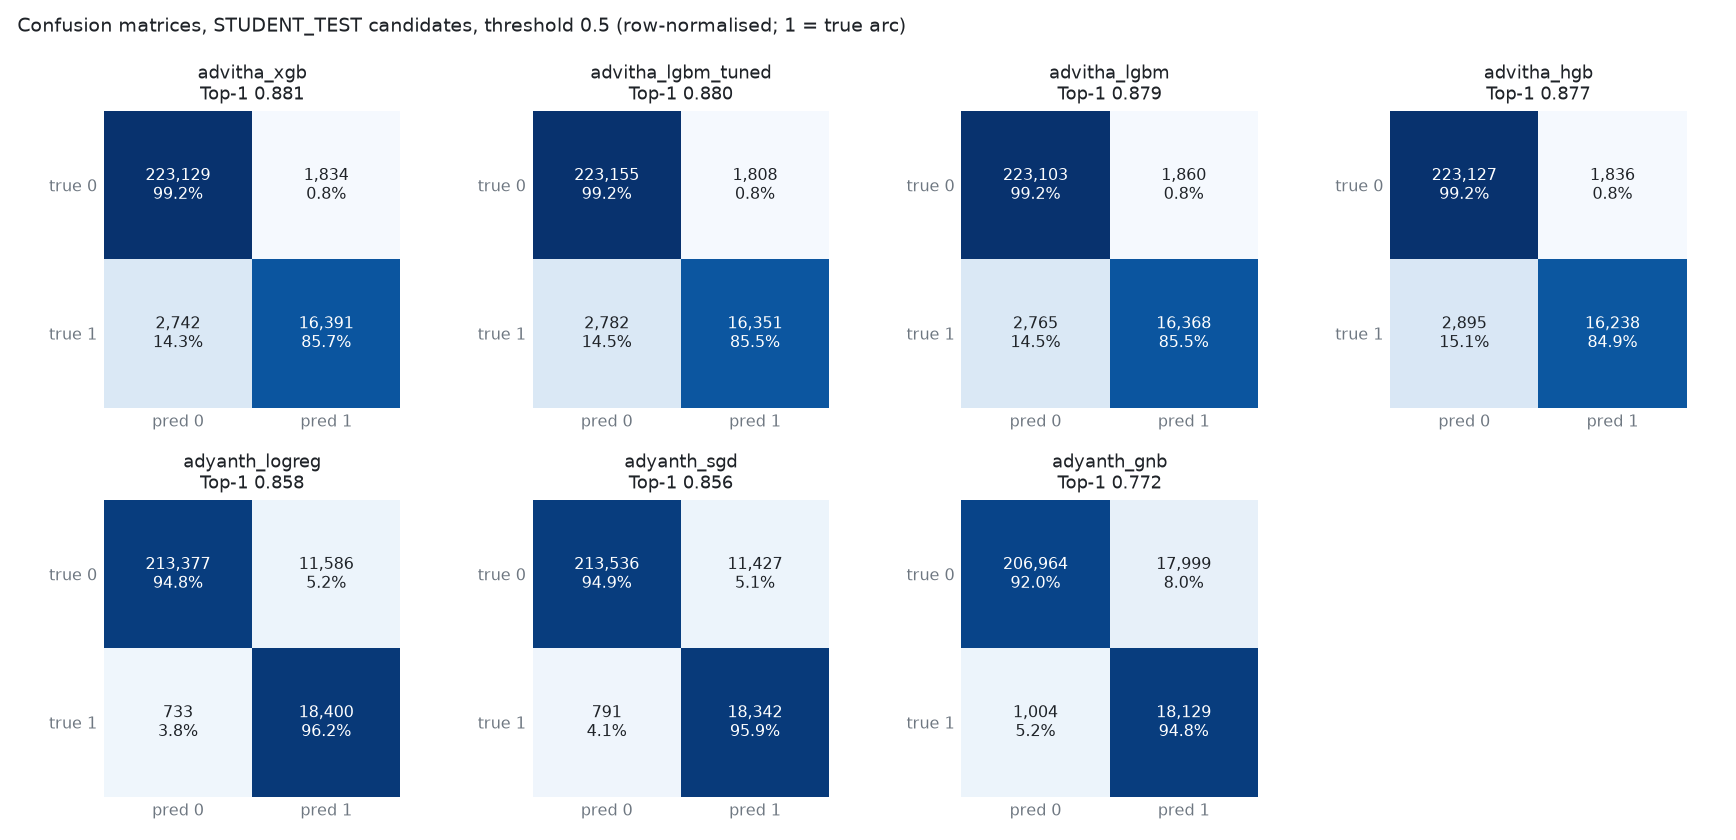
\includegraphics[width=\linewidth]{../experiments/figures/confusion_matrices.png}
\caption{STUDENT\_TEST confusion matrices (threshold 0.5, row-normalised; 1 = true arc).}\label{fig:cm}\end{figure}

\begin{figure}[H]\centering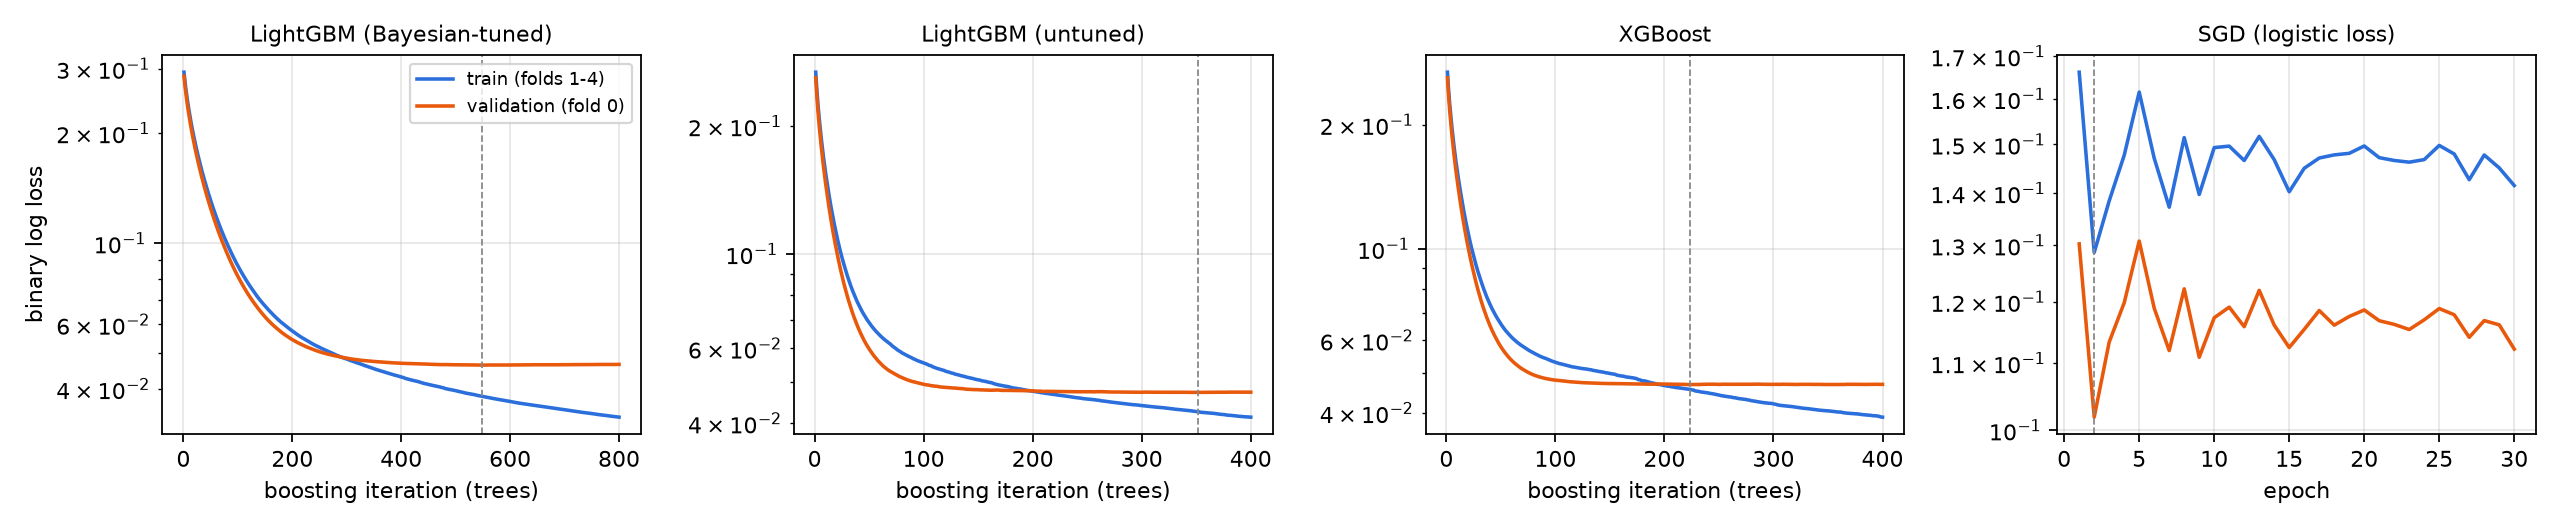
\includegraphics[width=\linewidth]{../experiments/figures/loss_curves.png}
\caption{Training and validation log loss per boosting iteration (LightGBM, XGBoost) and per epoch (SGD), CV fold 0 held out (\texttt{scripts/loss\_curves.py}). Dashed line: lowest validation loss.}\label{fig:loss}\end{figure}

Only boosting and SGD have a training history. Random Forest, Extra Trees and the Decision Tree are grown once,
Logistic Regression is solved to convergence by L-BFGS and Gaussian NB is fitted in closed form, so no loss curves are
drawn for them; their over/underfitting evidence is the train-fold vs CV gap in Table~\ref{tab:cv}.

\section{Bayesian hyperparameter optimisation}
\textbf{Model.} LightGBM, the best model before tuning. \textbf{Method.} Optuna's TPE sampler (multivariate, seed 148,
10 random start-up trials) with a median pruner.
\textbf{Q1--Q2. Search space}: Table~\ref{tab:space} (seven hyperparameters, log scale for the learning rate, number
of leaves, child size and regularisation).
\textbf{Q3. Objective}: mean CV Top-1 on TRAIN with the harness folds, the same as the selection metric; STUDENT\_TEST
was used once, after the search. Trial 0 was the untuned configuration, so the search starts at the baseline
(0.8639, identical to the harness).
\textbf{Q4. Trials}: 40 (40 complete, 0 pruned), 85 minutes on
8 CPU threads, 200 model fits; every trial is stored in \texttt{experiments/results/bayes\_opt/}.
\textbf{Q5. Best values}: Table~\ref{tab:space}, trial 32.

\begin{table}[H]\centering\small
\caption{Search space, best values (trial 32) and fANOVA importance.}\label{tab:space}
\resizebox{\ifdim\width>\linewidth\linewidth\else\width\fi}{!}{\begin{tabular}{lcccc}\toprule
Parameter & Range & Scale & Best & Importance \\ \midrule
n\_estimators & 200--1000 & uniform & 800 & 0.05 \\
learning\_rate & 0.01--0.2 & log & 0.01413 & 0.07 \\
num\_leaves & 15--255 & log & 254 & 0.70 \\
min\_child\_samples & 10--400 & log & 20 & 0.10 \\
subsample & 0.5--1.0 & uniform & 0.9151 & 0.01 \\
colsample\_bytree & 0.4--1.0 & uniform & 0.7893 & 0.02 \\
reg\_lambda & 0.001--30.0 & log & 0.04488 & 0.01 \\
reg\_alpha & 0.001--10.0 & log & 1.524 & 0.04 \\
\bottomrule\end{tabular}}\end{table}

\begin{table}[H]\centering\small
\caption{Untuned vs Bayesian-tuned LightGBM (same folds, features, seed).}\label{tab:tune}
\resizebox{\ifdim\width>\linewidth\linewidth\else\width\fi}{!}{\begin{tabular}{llrrr}\toprule
Metric & Partition & Untuned & Tuned & Change \\ \midrule
CV macro F1 (mean) & train CV & 0.9246 & 0.9253 & +0.0008 \\
CV macro F1 (std over folds) & train CV & 0.0184 & 0.0188 & +0.0004 \\
CV Top-1 (mean) & train CV & 0.8639 & 0.8651 & +0.0012 \\
CV log loss (mean) & train CV & 0.0637 & 0.0638 & +0.0001 \\
train-fold macro F1 (mean) & train CV & 0.9521 & 0.9634 & +0.0112 \\
Top-1 & student\_test & 0.8787 & 0.8796 & +0.0008 \\
macro F1 & student\_test & 0.9330 & 0.9334 & +0.0004 \\
log loss & student\_test & 0.0473 & 0.0470 & -0.0004 \\
route continuity (argmax) & student\_test & 0.8669 & 0.8666 & -0.0003 \\
final fit time (s) & train & 11.7036 & 40.8319 & +29.1282 \\
inference (ms per trip) & student\_test & 36.9916 & 169.1734 & +132.1818 \\
\bottomrule\end{tabular}}\end{table}

\begin{figure}[H]\centering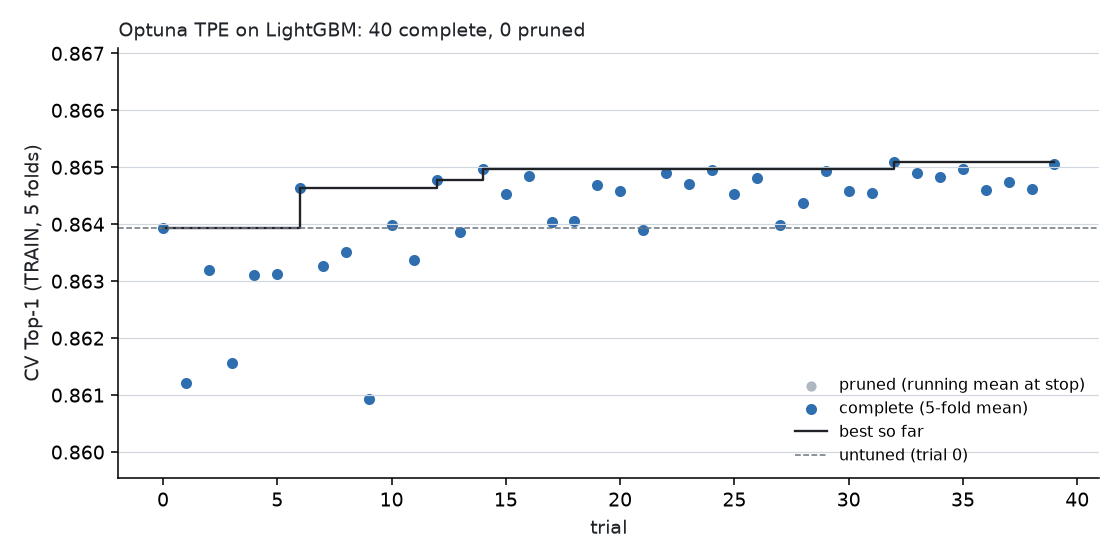
\includegraphics[width=0.8\linewidth]{../experiments/figures/bayes_opt_history.png}
\caption{Optimisation history: every trial, best so far, untuned baseline dashed.}\label{fig:bohist}\end{figure}

\textbf{Q6. Did tuning help?} Slightly, and consistently: CV Top-1 +0.0012 (better in 4 of 5 folds), STUDENT\_TEST
Top-1 +0.0008, log loss lower. The hand-picked defaults were already close to the optimum for these features. After the
random phase TPE converged on many leaves (about 200--255), a low learning rate and more trees; \texttt{num\_leaves}
explains about 70\% of the variation. The price is a 3.5$\times$ longer fit, 4.6$\times$ slower inference and a slightly
larger train/CV gap. The pruner never fired because all configurations score within 0.004 of each other.

\section{HMM and Viterbi route reconstruction}\label{sec:hmm}
\textbf{Q1. Hidden states.} At time $t$ the hidden states are the candidate arcs of point $t$ (a ragged set, at most 30).
\textbf{Q2. Emissions.} $\log e_t(a) = \operatorname{logsoftmax}_a\big(w \log \tilde p_t(a) + (1-w)\log
\mathcal{N}(d_t(a);0,\sigma)\big)$, where $\tilde p$ is the classifier probability normalised over the point's
candidates (floored at $10^{-6}$), $d$ the point-to-arc distance and $w$ the classifier weight.
\textbf{Q3. Transitions.} From arc $a$ at $t-1$ to arc $b$ at $t$ we compute the driving distance on the directed
network (rest of $a$, shortest path by Dijkstra from the end of $a$ to the start of $b$, part of $b$; along the arc for
a same-arc move) and compare it with the straight-line distance between the two GPS points:
$\log T(a\to b) = \operatorname{logsoftmax}_b\big(-|\text{route} - \text{straight}|/\beta\big)$. Paths longer than
$2\times$straight$+200$\,m are impossible ($-\infty$). This favours plausible connected paths and respects one-way arcs.
Viterbi runs in log space, $\delta_t(b) = \log e_t(b) + \max_a [\delta_{t-1}(a) + \log T(a\to b)]$, with back-pointers.
\textbf{Q4. Missing candidates and large gaps.} The chain is split when two points are more than
30\,s apart or when a point has no candidate; each piece is decoded on its own.
\textbf{Q5. Disconnected segments.} If no finite transition exists between two consecutive candidate sets (the roads
are not connected within the allowed detour), the chain is split there too, so every point with candidates still gets
an arc; the break is counted in the continuity metric.

\textbf{Tuning.} $w$ and $\beta$ were tuned on the 80 TRAIN trips only, with \emph{out-of-fold} classifier scores
(refitted without each fold), because in-sample scores are over-confident. Best: $w=1$,
$\beta=3$\,m (TRAIN Top-1 0.9198 vs 0.8654 for the argmax).

\begin{table}[H]\centering\small
\caption{HMM decoder grid on the 80 TRAIN trips with out-of-fold classifier scores (objective: Top-1).}\label{tab:grid}
\resizebox{\ifdim\width>\linewidth\linewidth\else\width\fi}{!}{\begin{tabular}{lccc}\toprule
Setting (w = classifier weight, $\beta$ in m) & Top-1 & Continuity & Route F1 \\ \midrule
w=1,beta=3 & 0.9198 & 0.9232 & 0.9014 \\
w=1,beta=5 & 0.9191 & 0.9259 & 0.9014 \\
w=1,beta=2 & 0.9179 & 0.9190 & 0.8998 \\
w=0.75,beta=5 & 0.9176 & 0.9232 & 0.9023 \\
w=0.75,beta=3 & 0.9171 & 0.9208 & 0.9018 \\
w=1,beta=10 & 0.9142 & 0.9262 & 0.8976 \\
w=0.75,beta=10 & 0.9131 & 0.9236 & 0.8996 \\
w=0.75,beta=2 & 0.9116 & 0.9150 & 0.8992 \\
w=0.5,beta=5 & 0.9111 & 0.9201 & 0.9023 \\
w=1,beta=20 & 0.9087 & 0.9256 & 0.8876 \\
w=0.5,beta=3 & 0.9078 & 0.9158 & 0.9007 \\
w=0.5,beta=10 & 0.9076 & 0.9204 & 0.9027 \\
w=0.75,beta=20 & 0.9069 & 0.9229 & 0.8918 \\
w=1,beta=50 & 0.9045 & 0.9229 & 0.8689 \\
w=1,beta=1 & 0.9038 & 0.9070 & 0.8952 \\
w=0.75,beta=50 & 0.9022 & 0.9199 & 0.8742 \\
w=0.5,beta=2 & 0.9015 & 0.9105 & 0.9002 \\
w=0.5,beta=20 & 0.9001 & 0.9167 & 0.8942 \\
w=0.5,beta=50 & 0.8940 & 0.9135 & 0.8798 \\
w=0.75,beta=1 & 0.8920 & 0.9028 & 0.8942 \\
w=0.5,beta=1 & 0.8787 & 0.9001 & 0.8931 \\
argmax & 0.8654 & 0.8544 & 0.7660 \\
\bottomrule\end{tabular}}\end{table}

\begin{table}[H]\centering\small
\caption{Classifier-only vs classifier + HMM on STUDENT\_TEST (final exported classifier).}\label{tab:hmm}
\resizebox{\ifdim\width>\linewidth\linewidth\else\width\fi}{!}{\begin{tabular}{lccccccc}\toprule
Method & Top-1 & Cont. & Breaks & Route P & Route R & Route F1 & Decode ms/trip \\ \midrule
classifier argmax (no HMM) & 0.8796 & 0.867 & 653 & 0.734 & 0.920 & 0.796 & 1 \\
HMM previous setting (w=1, beta=5) & 0.9102 & 0.931 & 249 & 0.932 & 0.915 & 0.920 & 1435 \\
HMM distance-only (w=0, beta=3) & 0.8504 & 0.906 & 341 & 0.964 & 0.895 & 0.927 & 1425 \\
HMM tuned on train (w=1, beta=3) & 0.9131 & 0.930 & 259 & 0.939 & 0.918 & 0.926 & 1435 \\
\bottomrule\end{tabular}}\end{table}

\textbf{Q6. Did the HMM improve the route?} Yes. End to end through the API code path, Top-1 rises from 88.0\%
to 91.3\%, continuity from 0.867 to 0.930, route breaks fall from
653 to 259, and route F1 rises sharply because the route stops flickering between arcs.
The HMM improves 8 of the 10 trips.

\textbf{Where it did not help.} Trips where it is worse: 00000040 (0.940 $\to$ 0.932), 00000091 (0.879 $\to$ 0.875). Distance-only emissions ($w=0$) are clearly worse
than the classifier on Top-1, so the classifier does most of the work and the HMM mainly removes isolated mistakes.
Decoding costs about 1.6\,s per trip (max 3.5\,s) against
0.21\,s without it, dominated by shortest-path searches.

\begin{table}[H]\centering\small
\caption{Per-trip Top-1 on STUDENT\_TEST.}\label{tab:pertrip}
\resizebox{\ifdim\width>\linewidth\linewidth\else\width\fi}{!}{\begin{tabular}{lccc}\toprule
Trip & Classifier only & + HMM (tuned) & Change \\ \midrule
00000000 & 0.951 & 0.964 & +0.014 \\
00000007 & 0.966 & 0.992 & +0.026 \\
00000009 & 0.864 & 0.866 & +0.002 \\
00000040 & 0.940 & 0.932 & -0.007 \\
00000052 & 0.935 & 0.962 & +0.027 \\
00000056 & 0.895 & 0.945 & +0.050 \\
00000065 & 0.898 & 0.906 & +0.008 \\
00000076 & 0.892 & 0.910 & +0.018 \\
00000077 & 0.735 & 0.827 & +0.092 \\
00000091 & 0.879 & 0.875 & -0.003 \\
\bottomrule\end{tabular}}\end{table}

\begin{figure}[H]\centering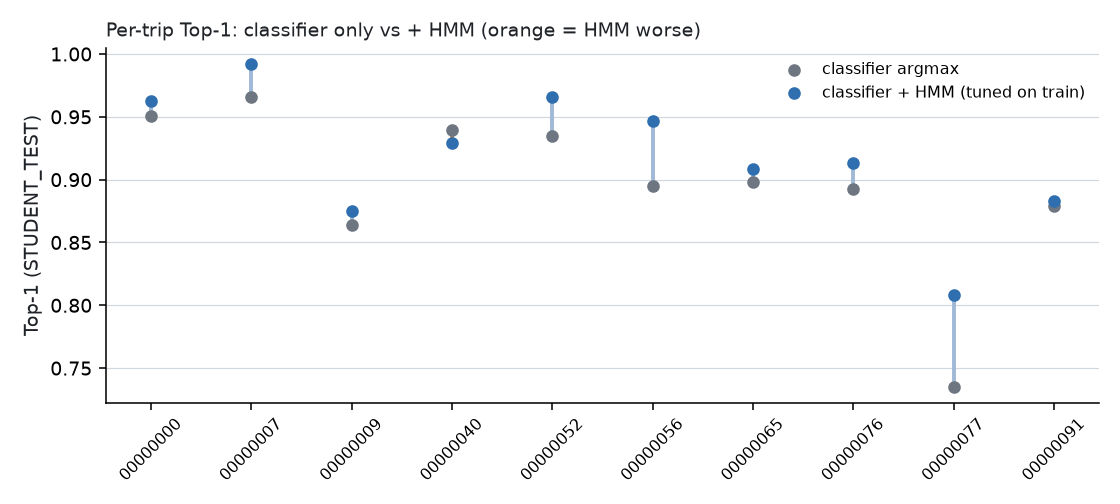
\includegraphics[width=0.85\linewidth]{../experiments/figures/hmm_comparison.png}
\caption{Per-trip Top-1 on STUDENT\_TEST, classifier only vs classifier + HMM.}\label{fig:hmmtrip}\end{figure}


\textbf{Failure analysis.} Of the 1,662 wrong points left, 877 are on an arc adjacent to the
label (sharing a junction) and 671 on the reverse direction of the label arc. Junction errors have a
median distance of about 8\,m to the shared node, inside GPS noise, where the label is set by where the alignment
switched arcs. Trip 00000077 alone holds 41\% of all errors, mostly reverse-direction ones; for
266 of the reverse errors the prediction agrees with the GPS heading while the label does
not, which points to direction noise in the reference route rather than in the model.

\section{Geographical visualisation with Folium}
\texttt{scripts/make\_maps.py} draws, for any trip, the raw GPS points, the road network within 200\,m of the track
(grey), the reference route (green, development trips only), the predicted route of the final pipeline (red), and GPS
points coloured blue where the predicted arc equals the label and orange where it differs, with a legend and a layer
control. The interactive HTML files are in \texttt{maps/}.
\begin{figure}[H]\centering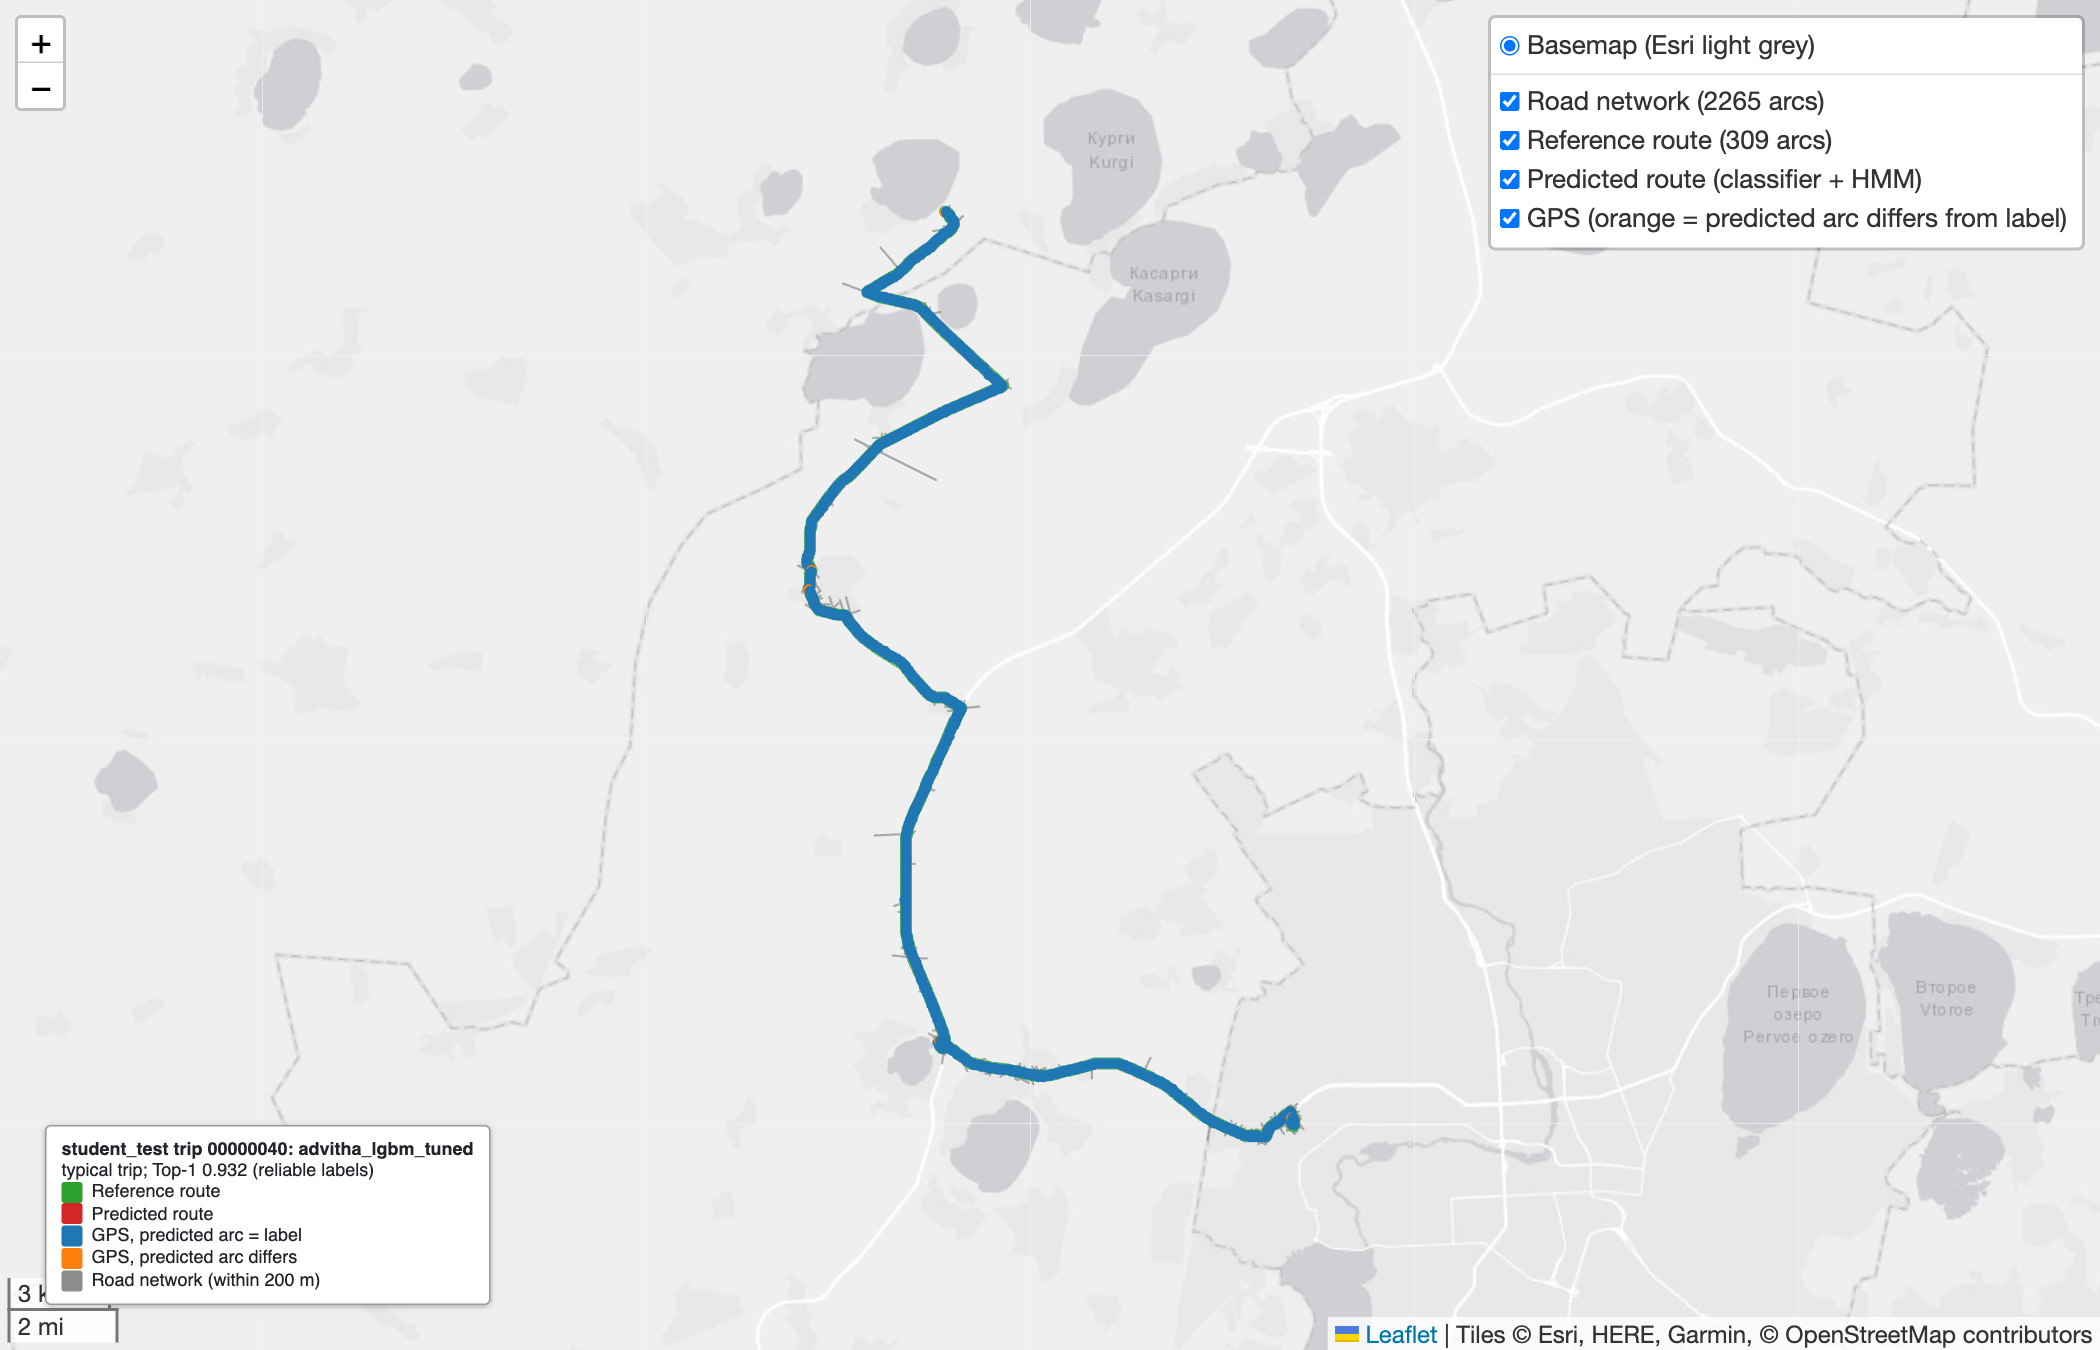
\includegraphics[width=0.85\linewidth]{figures/map_predicted_student_test_00000040.png}
\caption{STUDENT\_TEST trip 00000040: reference route vs route predicted by the final pipeline (tuned LightGBM + HMM).}\label{fig:map40}\end{figure}

\begin{figure}[H]\centering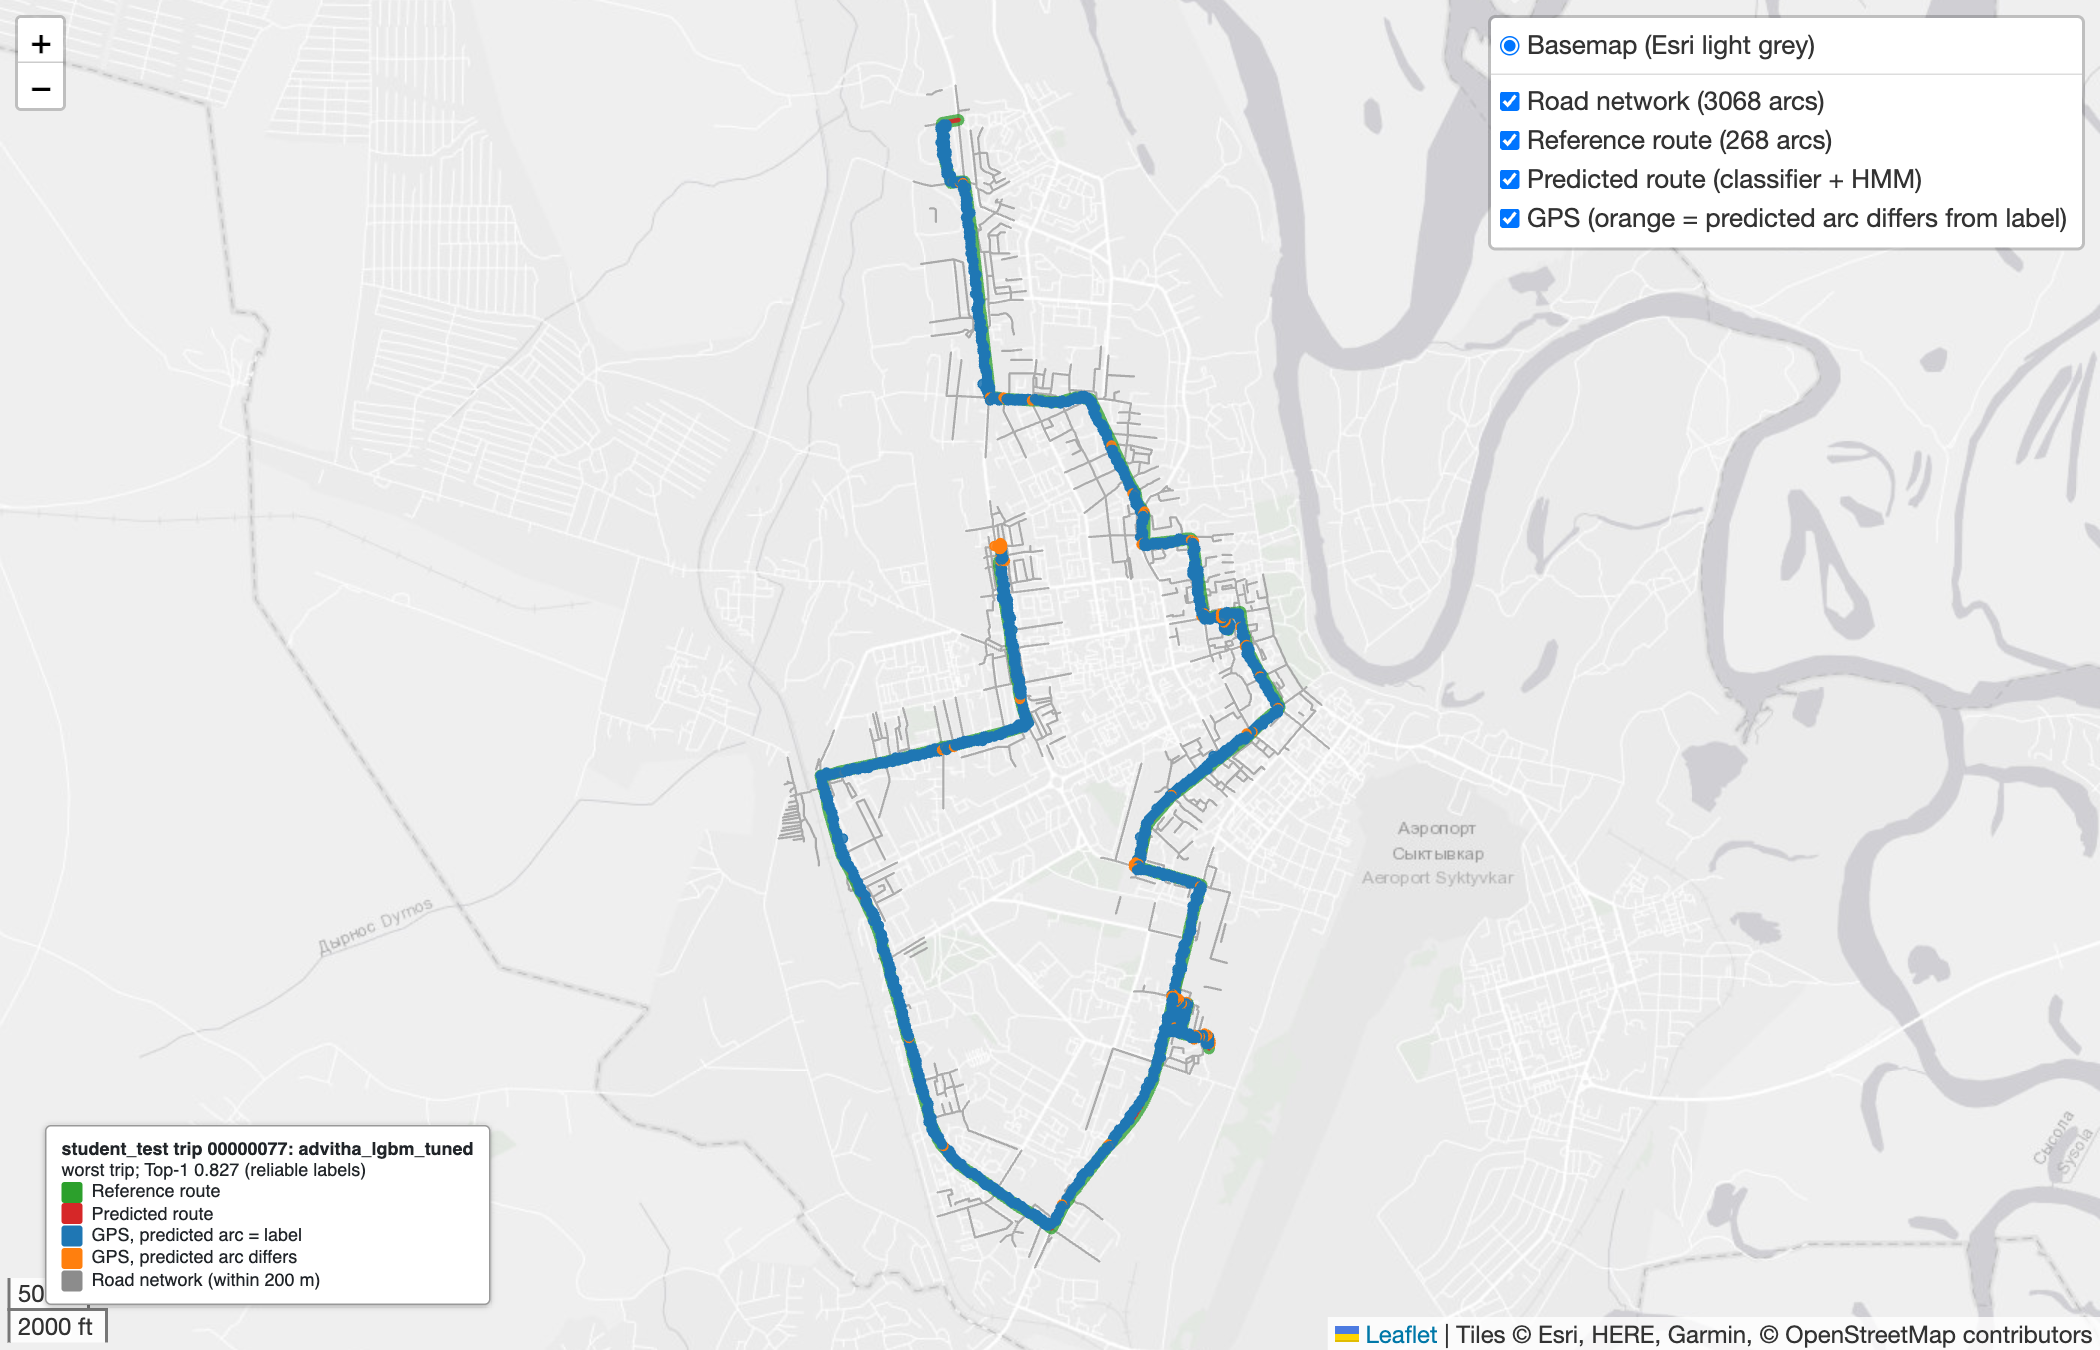
\includegraphics[width=0.85\linewidth]{figures/map_predicted_student_test_00000077.png}
\caption{STUDENT\_TEST trip 00000077, the hardest trip (final pipeline): most disagreements are on the reverse direction of the reference arc.}\label{fig:map77}\end{figure}


\section{API, UI and deployment}
\textbf{API (Laptop 1).} FastAPI (\texttt{scripts/run\_api.sh}, port 8000 on all interfaces) loads the classifier, the
HMM configuration and the trip files once at start-up. \texttt{/evaluator/trips} lists the evaluator trips and
\texttt{/evaluator/predict} runs the full pipeline on the track and network only. The reference route is read by
\texttt{api/evaluation.py} only \emph{after} prediction, to compute point Top-1 (labels from the same alignment as in
training), candidate miss rate, route precision/recall/F1, edit similarity and continuity. Only these numbers leave
the server; the reference route never reaches the model or the UI. Every request is logged with timings and scores.
\textbf{UI (Laptop 2).} Streamlit (\texttt{ui/app.py}) holds no data or model: it lists the evaluator trips, sends the
selected id and shows the predicted route on a Folium map with the server's scores.
\texttt{scripts/smoke\_test\_api.py} calls every evaluator trip: 10/10 passed, point-weighted Top-1 91.3\%
(Table~\ref{tab:eval}), in line with STUDENT\_TEST.

\begin{table}[H]\centering\small
\caption{Scores computed by the API server after prediction on the 10 EVALUATOR trips (\texttt{scripts/smoke\_test\_api.py}, log in Figure~\ref{fig:api}).}\label{tab:eval}
\resizebox{\ifdim\width>\linewidth\linewidth\else\width\fi}{!}{\begin{tabular}{lccccc}\toprule
Evaluator trip & Points scored & Top-1 & Miss rate & Route F1 & Continuity \\ \midrule
00000015 & 6,833 & 0.865 & 0.000 & 0.600 & 0.952 \\
00000017 & 1,346 & 0.874 & 0.000 & 0.854 & 0.804 \\
00000023 & 458 & 0.952 & 0.000 & 0.878 & 0.921 \\
00000030 & 654 & 0.813 & 0.000 & 0.814 & 0.824 \\
00000049 & 2,642 & 0.993 & 0.000 & 0.985 & 0.978 \\
00000059 & 1,031 & 0.908 & 0.000 & 0.888 & 0.845 \\
00000067 & 916 & 0.967 & 0.000 & 0.963 & 0.948 \\
00000073 & 1,144 & 0.971 & 0.000 & 0.981 & 0.970 \\
00000087 & 1,399 & 0.984 & 0.000 & 0.987 & 0.975 \\
00000094 & 3,230 & 0.915 & 0.000 & 0.907 & 0.917 \\
\bottomrule\end{tabular}}\end{table}

\begin{figure}[H]\centering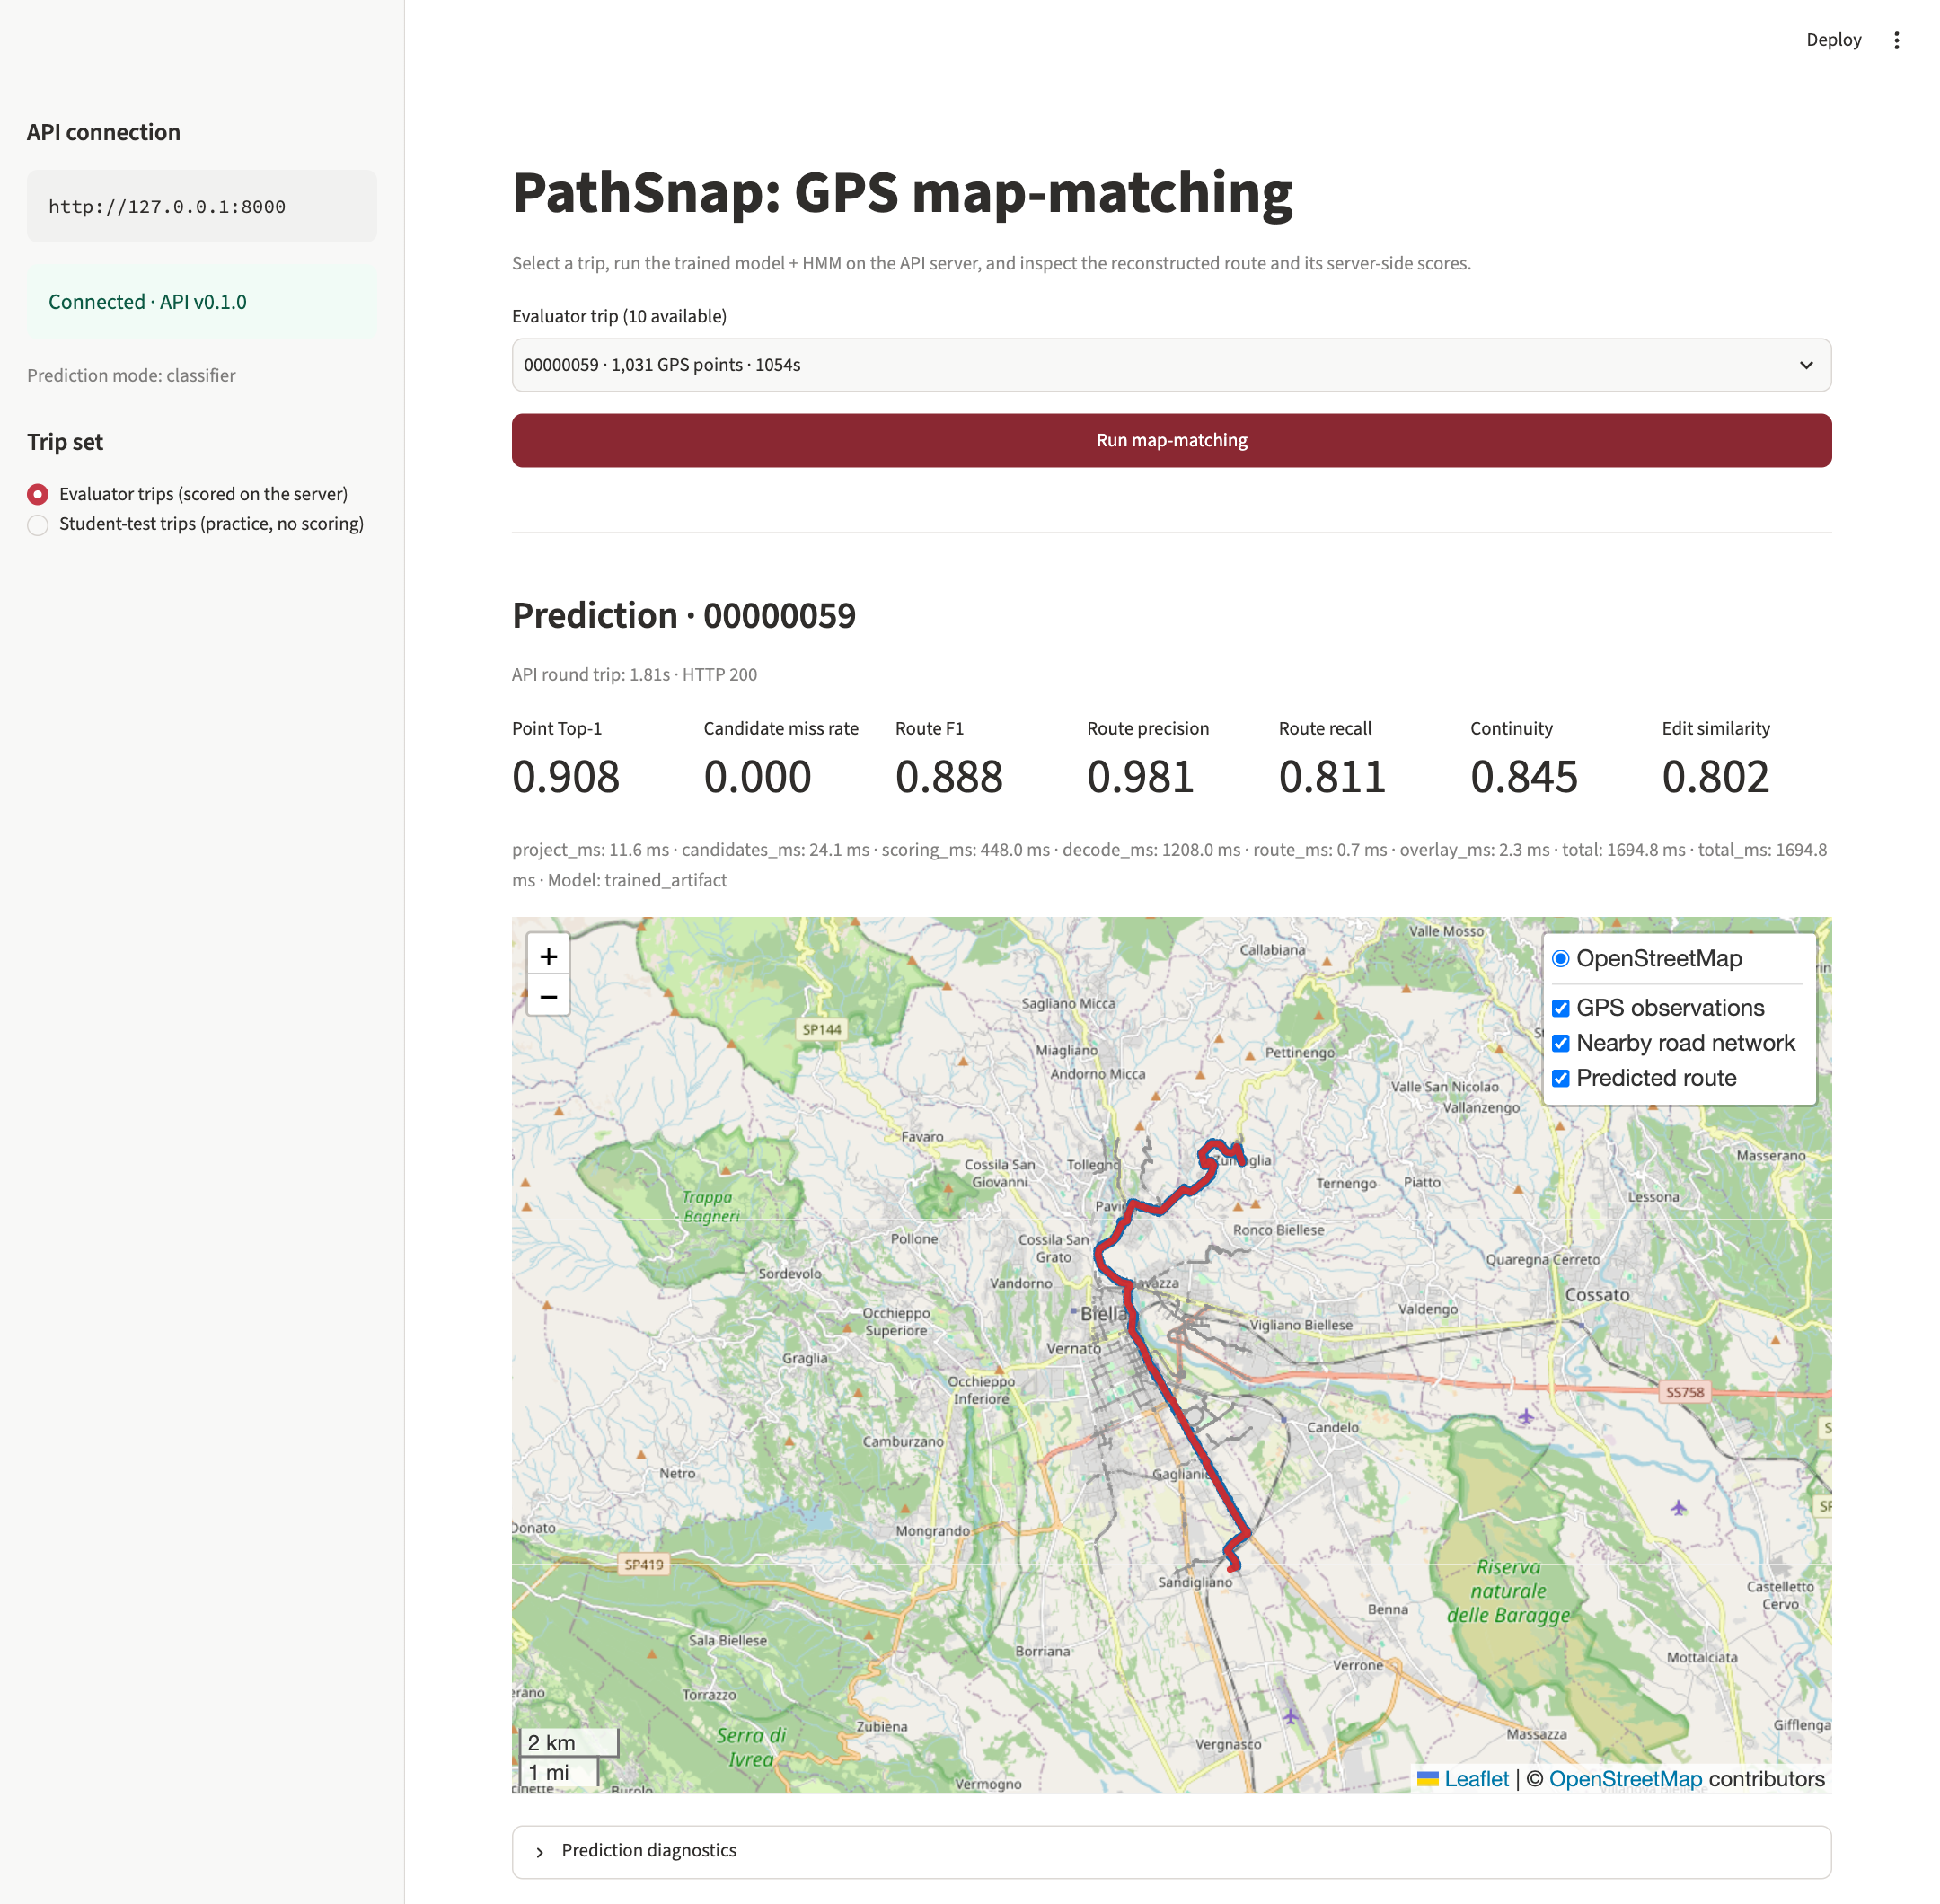
\includegraphics[width=0.8\linewidth]{figures/ui_evaluator.png}
\caption{UI showing evaluator trip 00000059: server-side scores and the predicted route.}\label{fig:ui}\end{figure}

\begin{figure}[H]\centering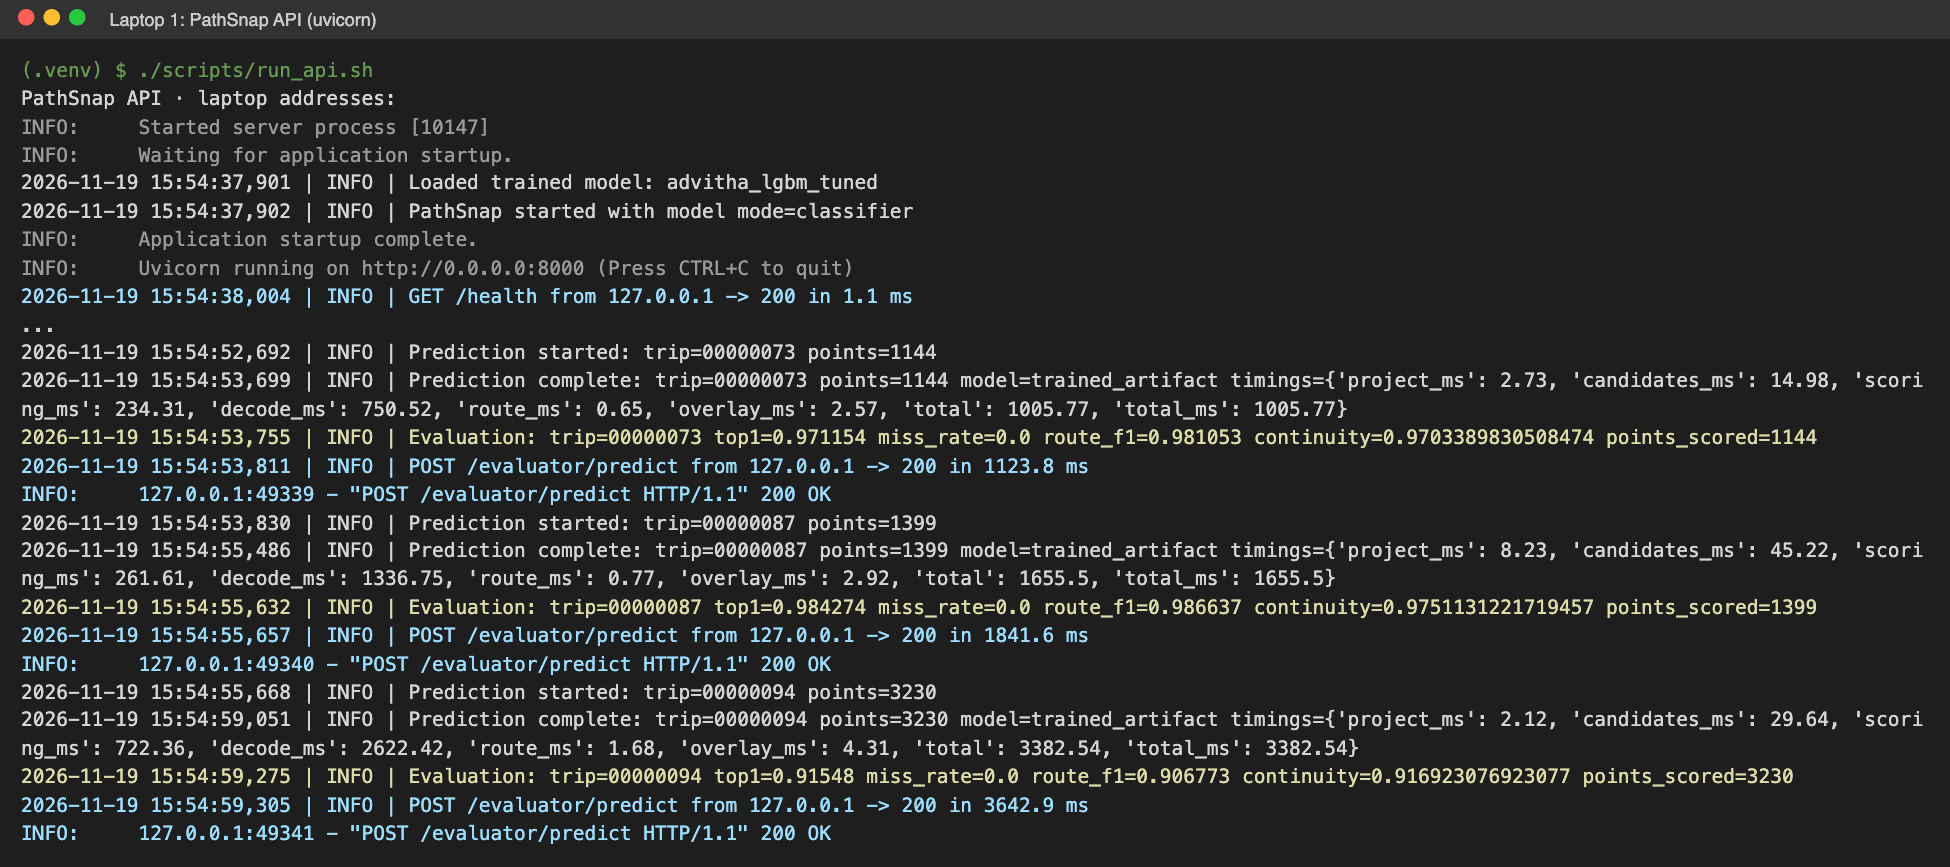
\includegraphics[width=\linewidth]{figures/api_terminal.png}
\caption{Terminal of the API server during the evaluator smoke test: requests, timings and server-side scores (the first lines are the start-up).}\label{fig:api}\end{figure}


\section{Academic integrity and AI use}
No evaluator data was used for training, feature selection, model choice, thresholds or decoder tuning; the loader
enforces this. There are no hard-coded predictions or trip-specific code paths. Every number in this report is read
from \texttt{experiments/results/} by \texttt{report/build\_report.py} and can be reproduced with the run order in the
README (seed 148). \textbf{AI assistance} was used for parts of the code and for drafting this report, under the team's
direction and as disclosed in \texttt{docs/AI\_USE.md}; all results come from running the repository's scripts, and
every member has reviewed the work.

\section{Limitations}
The per-point labels are derived, not given, and are uncertain at junctions and on two-way roads, so Top-1 is a
conservative measure. STUDENT\_TEST has only 10 trips, so differences below about one point are not meaningful. The HMM
decoder is roughly 8$\times$ slower than classifier-only inference, acceptable here (seconds per trip) but it would need
cached shortest paths at scale.

\end{document}
